%% This demo file is intended to serve as a ``starter file'' for 
%% IEEE Journal of Electromagnetics, RF and Microwaves in Medicine and
%% Biology (JERM) papers produced under \LaTeX\ using modified IEEEtran.cls
%% file in order to meet the special typesetting requirements of JERM.

%% Modified by Zhengyu Peng based on bare_jrnl.tex from Michael Shell 
%% Support sites:
%% https://github.com/rookiepeng/JERM-LaTeX-Template
%% http://www.michaelshell.org/tex/ieeetran/
%% http://www.ctan.org/pkg/ieeetran
%% and
%% http://www.ieee.org/

%%*************************************************************************
%% Legal Notice:
%% This code is offered as-is without any warranty either expressed or
%% implied; without even the implied warranty of MERCHANTABILITY or
%% FITNESS FOR A PARTICULAR PURPOSE! 
%% User assumes all risk.
%% In no event shall the IEEE or any contributor to this code be liable for
%% any damages or losses, including, but not limited to, incidental,
%% consequential, or any other damages, resulting from the use or misuse
%% of any information contained here.
%%
%% All comments are the opinions of their respective authors and are not
%% necessarily endorsed by the IEEE.
%%
%% This work is distributed under the LaTeX Project Public License (LPPL)
%% ( http://www.latex-project.org/ ) version 1.3, and may be freely used,
%% distributed and modified. A copy of the LPPL, version 1.3, is included
%% in the base LaTeX documentation of all distributions of LaTeX released
%% 2003/12/01 or later.
%% Retain all contribution notices and credits.
%% ** Modified files should be clearly indicated as such, including  **
%% ** renaming them and changing author support contact information. **
%%*************************************************************************

% *** Authors should verify (and, if needed, correct) their LaTeX system  ***
% *** with the testflow diagnostic prior to trusting their LaTeX platform ***
% *** with production work. The IEEE's font choices and paper sizes can   ***
% *** trigger bugs that do not appear when using other class files.       ***                          ***

\documentclass[journal,twocolumn,letterpaper]{IEEEJERM}
%
% If IEEEtran.cls has not been installed into the LaTeX system files,
% manually specify the path to it like:
% \documentclass[journal]{../sty/IEEEtran}

% Some very useful LaTeX packages include:
% (uncomment the ones you want to load)

% *** MISC UTILITY PACKAGES ***
%
%\usepackage{ifpdf}
% Heiko Oberdiek's ifpdf.sty is very useful if you need conditional
% compilation based on whether the output is pdf or dvi.
% usage:
% \ifpdf
%   % pdf code
% \else
%   % dvi code
% \fi
% The latest version of ifpdf.sty can be obtained from:
% http://www.ctan.org/pkg/ifpdf
% Also, note that IEEEtran.cls V1.7 and later provides a builtin
% \ifCLASSINFOpdf conditional that works the same way.
% When switching from latex to pdflatex and vice-versa, the compiler may
% have to be run twice to clear warning/error messages.


% *** CITATION PACKAGES ***
%
%\usepackage{cite}
% cite.sty was written by Donald Arseneau
% V1.6 and later of IEEEtran pre-defines the format of the cite.sty package
% \cite{} output to follow that of the IEEE. Loading the cite package will
% result in citation numbers being automatically sorted and properly
% "compressed/ranged". e.g., [1], [9], [2], [7], [5], [6] without using
% cite.sty will become [1], [2], [5]--[7], [9] using cite.sty. cite.sty's
% \cite will automatically add leading space, if needed. Use cite.sty's
% noadjust option (cite.sty V3.8 and later) if you want to turn this off
% such as if a citation ever needs to be enclosed in parenthesis.
% cite.sty is already installed on most LaTeX systems. Be sure and use
% version 5.0 (2009-03-20) and later if using hyperref.sty.
% The latest version can be obtained at:
% http://www.ctan.org/pkg/cite
% The documentation is contained in the cite.sty file itself.


% *** GRAPHICS RELATED PACKAGES ***
%
\ifCLASSINFOpdf
  % \usepackage[pdftex]{graphicx}
  % declare the path(s) where your graphic files are
  % \graphicspath{{../pdf/}{../jpeg/}}
  % and their extensions so you won't have to specify these with
  % every instance of \includegraphics
  % \DeclareGraphicsExtensions{.pdf,.jpeg,.png}
\else
  % or other class option (dvipsone, dvipdf, if not using dvips). graphicx
  % will default to the driver specified in the system graphics.cfg if no
  % driver is specified.
  % \usepackage[dvips]{graphicx}
  % declare the path(s) where your graphic files are
  % \graphicspath{{../eps/}}
  % and their extensions so you won't have to specify these with
  % every instance of \includegraphics
  % \DeclareGraphicsExtensions{.eps}
\fi
% graphicx was written by David Carlisle and Sebastian Rahtz. It is
% required if you want graphics, photos, etc. graphicx.sty is already
% installed on most LaTeX systems. The latest version and documentation
% can be obtained at: 
% http://www.ctan.org/pkg/graphicx
% Another good source of documentation is "Using Imported Graphics in
% LaTeX2e" by Keith Reckdahl which can be found at:
% http://www.ctan.org/pkg/epslatex
%
% latex, and pdflatex in dvi mode, support graphics in encapsulated
% postscript (.eps) format. pdflatex in pdf mode supports graphics
% in .pdf, .jpeg, .png and .mps (metapost) formats. Users should ensure
% that all non-photo figures use a vector format (.eps, .pdf, .mps) and
% not a bitmapped formats (.jpeg, .png). The IEEE frowns on bitmapped formats
% which can result in "jaggedy"/blurry rendering of lines and letters as
% well as large increases in file sizes.
%
% You can find documentation about the pdfTeX application at:
% http://www.tug.org/applications/pdftex


% *** MATH PACKAGES ***
%
%\usepackage{amsmath}
% A popular package from the American Mathematical Society that provides
% many useful and powerful commands for dealing with mathematics.
%
% Note that the amsmath package sets \interdisplaylinepenalty to 10000
% thus preventing page breaks from occurring within multiline equations. Use:
%\interdisplaylinepenalty=2500
% after loading amsmath to restore such page breaks as IEEEtran.cls normally
% does. amsmath.sty is already installed on most LaTeX systems. The latest
% version and documentation can be obtained at:
% http://www.ctan.org/pkg/amsmath


% *** SPECIALIZED LIST PACKAGES ***
%
%\usepackage{algorithmic}
% algorithmic.sty was written by Peter Williams and Rogerio Brito.
% This package provides an algorithmic environment fo describing algorithms.
% You can use the algorithmic environment in-text or within a figure
% environment to provide for a floating algorithm. Do NOT use the algorithm
% floating environment provided by algorithm.sty (by the same authors) or
% algorithm2e.sty (by Christophe Fiorio) as the IEEE does not use dedicated
% algorithm float types and packages that provide these will not provide
% correct IEEE style captions. The latest version and documentation of
% algorithmic.sty can be obtained at:
% http://www.ctan.org/pkg/algorithms
% Also of interest may be the (relatively newer and more customizable)
% algorithmicx.sty package by Szasz Janos:
% http://www.ctan.org/pkg/algorithmicx


% *** ALIGNMENT PACKAGES ***
%
%\usepackage{array}
% Frank Mittelbach's and David Carlisle's array.sty patches and improves
% the standard LaTeX2e array and tabular environments to provide better
% appearance and additional user controls. As the default LaTeX2e table
% generation code is lacking to the point of almost being broken with
% respect to the quality of the end results, all users are strongly
% advised to use an enhanced (at the very least that provided by array.sty)
% set of table tools. array.sty is already installed on most systems. The
% latest version and documentation can be obtained at:
% http://www.ctan.org/pkg/array


% IEEEtran contains the IEEEeqnarray family of commands that can be used to
% generate multiline equations as well as matrices, tables, etc., of high
% quality.


% *** SUBFIGURE PACKAGES ***
%\ifCLASSOPTIONcompsoc
%  \usepackage[caption=false,font=normalsize,labelfont=sf,textfont=sf]{subfig}
%\else
%  \usepackage[caption=false,font=footnotesize]{subfig}
%\fi
% subfig.sty, written by Steven Douglas Cochran, is the modern replacement
% for subfigure.sty, the latter of which is no longer maintained and is
% incompatible with some LaTeX packages including fixltx2e. However,
% subfig.sty requires and automatically loads Axel Sommerfeldt's caption.sty
% which will override IEEEtran.cls' handling of captions and this will result
% in non-IEEE style figure/table captions. To prevent this problem, be sure
% and invoke subfig.sty's "caption=false" package option (available since
% subfig.sty version 1.3, 2005/06/28) as this is will preserve IEEEtran.cls
% handling of captions.
% Note that the Computer Society format requires a larger sans serif font
% than the serif footnote size font used in traditional IEEE formatting
% and thus the need to invoke different subfig.sty package options depending
% on whether compsoc mode has been enabled.
%
% The latest version and documentation of subfig.sty can be obtained at:
% http://www.ctan.org/pkg/subfig


% *** FLOAT PACKAGES ***
%
%\usepackage{fixltx2e}
% fixltx2e, the successor to the earlier fix2col.sty, was written by
% Frank Mittelbach and David Carlisle. This package corrects a few problems
% in the LaTeX2e kernel, the most notable of which is that in current
% LaTeX2e releases, the ordering of single and double column floats is not
% guaranteed to be preserved. Thus, an unpatched LaTeX2e can allow a
% single column figure to be placed prior to an earlier double column
% figure.
% Be aware that LaTeX2e kernels dated 2015 and later have fixltx2e.sty's
% corrections already built into the system in which case a warning will
% be issued if an attempt is made to load fixltx2e.sty as it is no longer
% needed.
% The latest version and documentation can be found at:
% http://www.ctan.org/pkg/fixltx2e


%\usepackage{stfloats}
% stfloats.sty was written by Sigitas Tolusis. This package gives LaTeX2e
% the ability to do double column floats at the bottom of the page as well
% as the top. (e.g., "\begin{figure*}[!b]" is not normally possible in
% LaTeX2e). It also provides a command:
%\fnbelowfloat
% to enable the placement of footnotes below bottom floats (the standard
% LaTeX2e kernel puts them above bottom floats). This is an invasive package
% which rewrites many portions of the LaTeX2e float routines. It may not work
% with other packages that modify the LaTeX2e float routines. The latest
% version and documentation can be obtained at:
% http://www.ctan.org/pkg/stfloats
% Do not use the stfloats baselinefloat ability as the IEEE does not allow
% \baselineskip to stretch. Authors submitting work to the IEEE should note
% that the IEEE rarely uses double column equations and that authors should try
% to avoid such use. Do not be tempted to use the cuted.sty or midfloat.sty
% packages (also by Sigitas Tolusis) as the IEEE does not format its papers in
% such ways.
% Do not attempt to use stfloats with fixltx2e as they are incompatible.
% Instead, use Morten Hogholm'a dblfloatfix which combines the features
% of both fixltx2e and stfloats:
%
% \usepackage{dblfloatfix}
% The latest version can be found at:
% http://www.ctan.org/pkg/dblfloatfix


%\ifCLASSOPTIONcaptionsoff
%  \usepackage[nomarkers]{endfloat}
% \let\MYoriglatexcaption\caption
% \renewcommand{\caption}[2][\relax]{\MYoriglatexcaption[#2]{#2}}
%\fi
% endfloat.sty was written by James Darrell McCauley, Jeff Goldberg and 
% Axel Sommerfeldt. This package may be useful when used in conjunction with 
% IEEEtran.cls'  captionsoff option. Some IEEE journals/societies require that
% submissions have lists of figures/tables at the end of the paper and that
% figures/tables without any captions are placed on a page by themselves at
% the end of the document. If needed, the draftcls IEEEtran class option or
% \CLASSINPUTbaselinestretch interface can be used to increase the line
% spacing as well. Be sure and use the nomarkers option of endfloat to
% prevent endfloat from "marking" where the figures would have been placed
% in the text. The two hack lines of code above are a slight modification of
% that suggested by in the endfloat docs (section 8.4.1) to ensure that
% the full captions always appear in the list of figures/tables - even if
% the user used the short optional argument of \caption[]{}.
% IEEE papers do not typically make use of \caption[]'s optional argument,
% so this should not be an issue. A similar trick can be used to disable
% captions of packages such as subfig.sty that lack options to turn off
% the subcaptions:
% For subfig.sty:
% \let\MYorigsubfloat\subfloat
% \renewcommand{\subfloat}[2][\relax]{\MYorigsubfloat[]{#2}}
% However, the above trick will not work if both optional arguments of
% the \subfloat command are used. Furthermore, there needs to be a
% description of each subfigure *somewhere* and endfloat does not add
% subfigure captions to its list of figures. Thus, the best approach is to
% avoid the use of subfigure captions (many IEEE journals avoid them anyway)
% and instead reference/explain all the subfigures within the main caption.
% The latest version of endfloat.sty and its documentation can obtained at:
% http://www.ctan.org/pkg/endfloat
%
% The IEEEtran \ifCLASSOPTIONcaptionsoff conditional can also be used
% later in the document, say, to conditionally put the References on a 
% page by themselves.


% *** PDF, URL AND HYPERLINK PACKAGES ***
%
%\usepackage{url}
% url.sty was written by Donald Arseneau. It provides better support for
% handling and breaking URLs. url.sty is already installed on most LaTeX
% systems. The latest version and documentation can be obtained at:
% http://www.ctan.org/pkg/url
% Basically, \url{my_url_here}.


% *** Do not adjust lengths that control margins, column widths, etc. ***
% *** Do not use packages that alter fonts (such as pslatex).         ***
% There should be no need to do such things with IEEEtran.cls V1.6 and later.
% (Unless specifically asked to do so by the journal or conference you plan
% to submit to, of course. )


\usepackage{times,amsmath,epsfig}
\usepackage{fancyhdr}
\usepackage{amsmath}
\usepackage{amsfonts}
\usepackage{amssymb}
\usepackage[utf8]{inputenc} %%% changed from latin1 to utf8
\usepackage{array}
\usepackage{graphicx}
\usepackage{url}
\usepackage{subfigure}
\usepackage{bm}
\usepackage{breqn}
\usepackage{xcolor}
\usepackage{soul}
\usepackage{amssymb}
\usepackage{makecell} % for \Xhline{2\arrayrulewidth}

%%% Added by me
\usepackage[serbian]{babel}
% \usepackage[utf8]{inputenc}


% correct bad hyphenation here
\hyphenation{op-tical net-works semi-conduc-tor}

\newcommand{\HRule}{\rule{\linewidth}{0.3mm}} % Defines a new command for the horizontal lines, changes thickness here


\begin{document}

%
% paper title
% Titles are generally capitalized except for words such as a, an, and, as,
% at, but, by, for, in, nor, of, on, or, the, to and up, which are usually
% not capitalized unless they are the first or last word of the title.
% Linebreaks \\ can be used within to get better formatting as desired.
% Do not put math or special symbols in the title.
\title{6-bitni aktivni pomerač faze - vektor modulator za opseg učestanosti oko 28 GHz -a}

%
% author names and IEEE memberships
% note positions of commas and nonbreaking spaces ( ~ ) LaTeX will not break
% a structure at a ~ so this keeps an author's name from being broken across
% two lines.
\author{Vuković Aleksandar 2018/3034, \textit{student} % <-this % stops a space
}% <-this % stops a space

% The paper headers
\markboth{Univerzitet u Beogradu, Elektrotehnički fakultet, Integrisana kola za komunikacione sisteme 13M041IKS}
{Z. Peng \MakeLowercase{\textit{et al.}}: Demo of IEEE Journal of Electromagnetics, RF and Microwaves in Medicine and Biology (JERM)}


% Mozda Vam bude interesantna tema pomeraca faze, konkretno vektor modulatora.
% Teoriju o pomeracima faze mozete naci u disertaciji:
% https://escholarship.org/content/qt8zz9v532/qt8zz9v532.pdf
% Poglavlje 2 se bavi vektor modulatorima, mada bi bilo dobro da pogledate i ostala poglavlja.

% Nesto novija referenca:
% https://www.jstage.jst.go.jp/article/elex/14/13/14_14.20170451/_pdf

% Ukoliko Vam je ova tema interesanta, predlozio bih da probate da napravite vektorski modulator koji bi pokrivao 28 i 38 GHz opsege. Ukoliko to nije moguce, fokusirajte se na 28 GHz.
% Probajte da dobijete 6b rezolucije, ali i 5b je sasvim prihvatljivo.

% Za digitalnu kontrolu bice Vam potreban D/A konvertor.
% Predlozio bih da koristite arhitekturu:
% https://web.engr.oregonstate.edu/~moon/research/files/cas2_may_05.pdf
% Mozete , ali ne morate da pravite 10b D/A, i 8b je sasvim dovoljno.

% Prvi projekat bi trebalo da bude pregled teorije i brza provera performansi kljucnih blokova, npr. QAF.
% U okviru drugog projekta biste mogli da se pozabavite tranzistorskom implementacijom.


\twocolumn[
\begin{@twocolumnfalse}
  
% make the title area
\maketitle

% As a general rule, do not put math, special symbols or citations
% in the abstract or keywords.
\begin{abstract}
U nastavku su predstavljeni blokovi aktivnog pomerača faze sa vektorskim modulatorom za tehnologiju IHP SiGe BiCMOS 130nm za opseg učestanosti oko 28 GHz (od 26.5 GHz do 29.5 GHz). Pomerač faze je kontrolisan 8-bitnim digitalno analognim konvertorom.
\end{abstract}

% Note that keywords are not normally used for peerreview papers.
% \begin{IEEEkeywords}
% IEEE, IEEEtran, journal, \LaTeX, paper, template.
% \end{IEEEkeywords}

\end{@twocolumnfalse}]

% Put footnotes here
% {
%   \renewcommand{\thefootnote}{}%
%   \footnotetext[1]{Authors' affiliation 1}
%   \footnotetext[2]{Authors' affiliation 2}
% }
 
% For peer review papers, you can put extra information on the cover
% page as needed:
% \ifCLASSOPTIONpeerreview
% \begin{center} \bfseries EDICS Category: 3-BBND \end{center}
% \fi
%
% For peerreview papers, this IEEEtran command inserts a page break and
% creates the second title. It will be ignored for other modes. 

\IEEEpeerreviewmaketitle

\section{Uvod}

\IEEEPARstart{N}{ajčešći} integrisani fazni pomerači se zasnivaju na vektor-modulatoru, topologiji sa raspoređenim parametrima (distribuirani) kao i topologijama reflektivnog i prekidačkog tipa. U nastavku je prikazan integrisani aktivni fazni pomerač zasnovan na vektor modulatoru. 

\subsection{Specifikacije pomerača faze}

Za razvoj i optimizaciju pomerača, potrebno je voditi računa o mnogobrojnim ograničenjima, od kojih treba izdvojiti:

\begin{itemize}

	\item opseg kontrole faze, teži $360^o$.
	\item fazna rezolucija, gde je poželjna linearna kontrola
	\item grupno kašnjenje, ima veliki uticaj na širokopojasne sisteme jer dovodi do disperzije (rasprašivanja)
	\item slabljenje signala, koje zavisi i od faze, ova zavisnost od faze se može nadoknaditi pojačavačima sa podesivim pojačanjem

\end{itemize}

ali i ne zanemariti sveprisutne zahteve vezane za širokopojasnost, linearnost kod velikog signala, potrošnju, prostor na čipu, šum i stabilnost sistema. Ove specifikacije se moraju razmatrati za sve topologije pomerača zasebno, zbog različitih podblokova.

\subsection{Arhitektura pomerača faze sa vektor modulatorom}

\begin{figure}[!htbp]
  \centering
  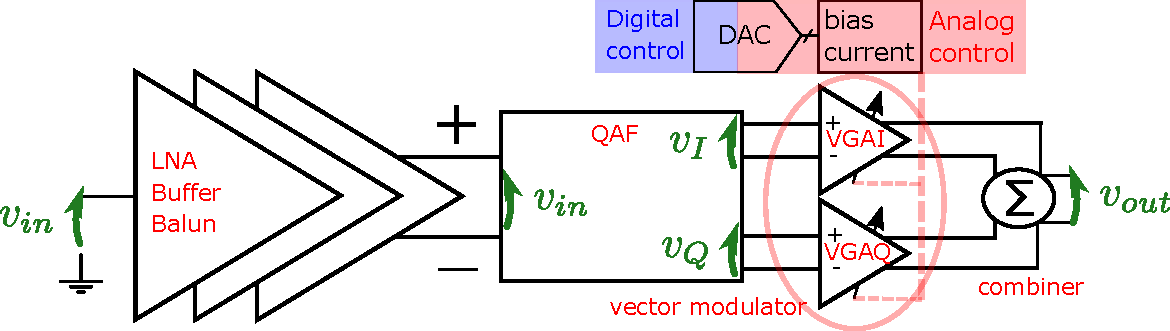
\includegraphics[width=\linewidth]{pshift_arch2.pdf}
  \caption{Arhitektura aktivnog faznog pomerača}
  \label{fig:pshift_arch}
\end{figure}

% TODO: dodati blok shemu i objašnjenje

Pomeranje faze, tj. sinteza faze se ostvaruje i zasnovana je na sabiranju kvadraturnih vektora linearnom operacijom koja je u idealnom slučaju nezavisna od učestanosti u određenom opsegu učestanosti. Digitalna kotrola pomeraja faze može biti implementirana direktno kao bit znaka I i Q signala koji se pojavljaju na ulazu pojačavača ili indirektno preko DA konvertora kojim se upravlja polarizacija tih pojačavača podesivih pojačanja (VGA), tako što će bit najveće težine postati bit znaka. U ovoj arhitekturi je iskorišćeno indirektno ostvarivanje ove kontrole znaka ulaznih signala vektor modualtora  Kako bi se lako izvršila promena znaka ulaznog signala on se prethodno prevodi u diferencijalni oblik pomoću \textit{BALUN}-a, da bi se potom I/Q \textit{all-pass} filtrom generisali signali u kvadraturi. Arhitektura aktivnog faznog pomerača je prikazana na slici ~\ref{fig:pshift_arch}.\cite{ellinger10}

Operacijom sabiranja dva signala u kvadraturi može se dostići fazni opseg od $90^o$, a operacijama sabiranjem i negiranjem se ostvaruje fazni opseg $360^o$.
% Ovo se može
% fazorski odnosi bi mogli da se prikažu radi vizuelizacije

% \begin{equation}
%   \label{eqn:trig}
%   cos(\alpha) + cos(\beta) = 2cos(\dfrac{\alpha + \beta}{2})cos(\dfrac{\alpha - \beta}{2})
% \end{equation}

% \begin{align}
%   \label{eqn:iq_signals}
%   \begin{split}
%     v_i(t) = A_I cos(\omega t), \\
%     v_q(t) = A_Q cos(\omega t + \dfrac{\pi}{4}); \\
%     \end{split}
% \end{align}

% \begin{equation}
%   \label{eqn:iq_sum}
%   v_i(t) + v_q(t) =  A_I cos(\omega t) cos(\omega t + \dfrac{\pi}{4})+ (A_Q - A_I)cos(\omega t)
% \end{equation}



Pošto se pojačavačem podesivog pojačanja upravlja DA konvertorom, fazna rezolucija pomerača faze je ograničena brojem bitova tog konvertora, ali ovaj broj se može degradirati i samom degradacijom signala koje modulišemo. \\


% Koliko veliki kalem mi treba kod vektor modulatora prema napajanju?

% Da li je potrebno prilagođenje između npr. bafera i baluna?

% Kako da ostvarim kombajner na ovom kolu (ne sme da bude mnogo kapacitvan)?\\



% The active phase shifter architecture is presented in Fig. 2.1. An I/Q network and two
% variable gain amplifiers (VGAs) are used in a differential mode for sign reversal, and the VGA
% outputs are summed in the current domain to create the final vector with arbitrary phase shift.
% The output phase relies on the gain ratio between the I- and Q-paths, and this results in a robust
% design against process, supply voltage and temperature variations. Phase synthesis based on
% the interpolation of quadrature vectors is a linear operation and is independent of frequency,
% guaranteeing wideband operation. The fundamental limitation of the phase accuracy and the
% operating bandwidth is given by the quadrature network.


% The very first letter is a 2 line initial drop letter followed
% by the rest of the first word in caps.
% 
% form to use if the first word consists of a single letter:
% \IEEEPARstart{A}{demo} file is ....
% 
% form to use if you need the single drop letter followed by
% normal text (unknown if ever used by the IEEE):
% \IEEEPARstart{A}{}demo file is ....
% 
% Some journals put the first two words in caps:
% \IEEEPARstart{T}{his demo} file is ....
% 
% Here we have the typical use of a "T" for an initial drop letter
% and "HIS" in caps to complete the first word.

% \IEEEPARstart{O}{vaj} projekat podrazumeva modelovanje pojačavača sa zadatim bipolarnim tranzistorom \textit{Philips (NXP) NPN BJT 6 GHz Wideband (BFR93A, SOT23) } i zadatom mirnom radnom tačkom gde su $V_{CE} = 8 V $, a $I_C = 20 mA $ dok je napajanje $ V_{CC} = 15 V $. U simulaciji se koriste \textbf{S}-parametri koje je zadao proizvođač. Zahtevi za rad pojačavača su da je stabilan u celom frekvencijskom opsegu, a pogonsko pojačanje $ G_T > 9 dB $ kao i da su koeficijenti stojećih talasa na ulazu i izlazu manji od $ 1,6 $. 


% You must have at least 2 lines in the paragraph with the drop letter
% (should never be an issue)
% I wish you the best of success.

% \hfill Z. Peng
 
% \hfill Jun 30, 2017


\section{Generator signala u kvadraturi}

Generator I/Q signala je ključan za rad faznog pomerača, jer od njegovih performansi zavisi preciznost faze, a time i kvalitet fazne modulacije. Važne specifikacije I/Q generatora su fazno i ampltitudsko odstupanje ova dva signala u kvadraturi, njihovo slabljenje i propusni opseg, od kojih su opseg i fazno odstupanje fundamentalna ograničenja. 

% The I/Q generation block is a critical part in a vector summing phase shifter, as its performance has a big effect on the phase interpolation quality. Its key performance
% specs include quadrature phase and amplitude accuracies, signal loss and band-
% width. In RF frequency bands, RC-CR pair and its poly-phase filter are commonly
% used to generate the quadrature signals. However, they suffer from inherent signal
% loss and sensitivity to process variations. In addition, differential quadrature vectors
% are needed to synthesize all four quadrant phases.

\subsection{RC-CR filtar}

\begin{figure}[!htbp]
  \centering
  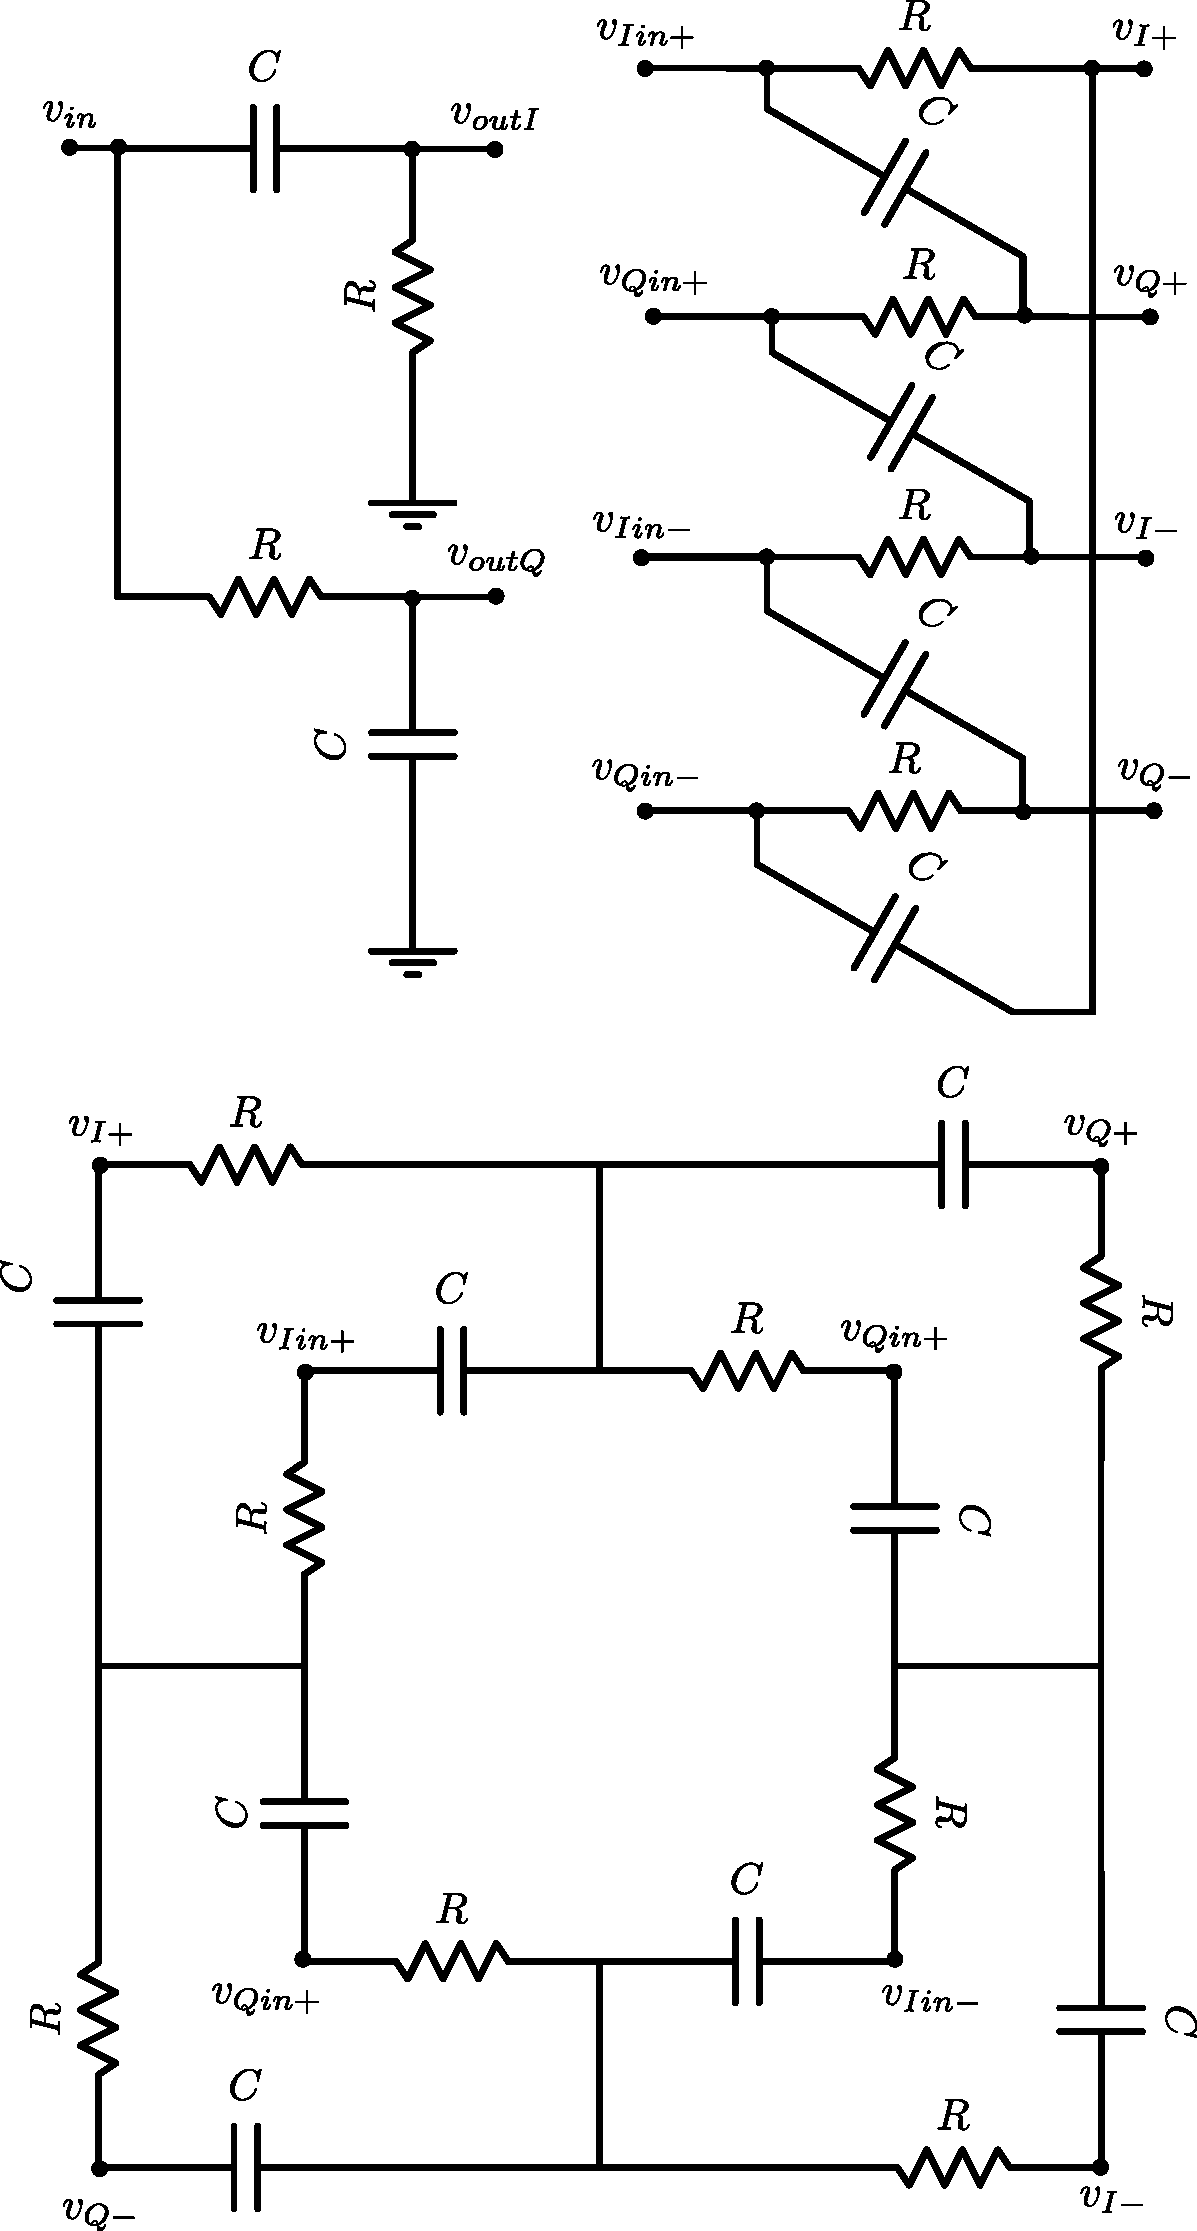
\includegraphics[width=0.8\linewidth]{rc_cr_single_multistage.pdf}
  \caption{RC-CR filtar kao i polifazna i višestepena verzija}
  \label{fig:rc_rc_single}
\end{figure}

Kao jednostavan primer I/Q generatora je predstavljen RC-CR filtar i njegova polifazna verzija. Kod ovog filtra se javlja problem slabljenja i osetljivosti na varijacije procesa. Izlazna impedansa filtra je kapacitivna, pa dodavanjem na izlaz kola čija kapacitivnost je obično istog reda kao i ova kapacitivnost, što se odražava kao izrazito uskopojasno ponašanje ovog filtra koje ograničava mogućnosti pomerača faze, iako sam po sebi za fazni pomeraj nema izraženu zavisnost od učestanosti. RC filtar i njegova polifazna kombinacija su prikazani na sl.~\ref{fig:rc_rc_single}.

Problem uskopojasnosti se na štetu povećanog slabljenja signala može ublažiti korišćenjem višestepenog polifazni RC-CR filtar. Ovakav filtar je korišćen za implementaciju u radu koji radi na učestanosti od 1 GHz. Višestepeni filtar je prikazan na sl.~\ref{fig:rc_rc_single}, i ima konstantu razliku faza na nekoliko oktava opsega učestansoti, pa se koristi za širokopojasna spread-spectrum rešenja \cite{chua98}.

\subsection{Kvadraturni \textit{all-pass} filtar (QAF)}

Kvadraturni \textit{all-pass} filtar (prikazan na sl.~\ref{fig:qaf_single_ended} zajedno sa fazorskim dijagramom)

\begin{figure}[!htbp]
  \centering
  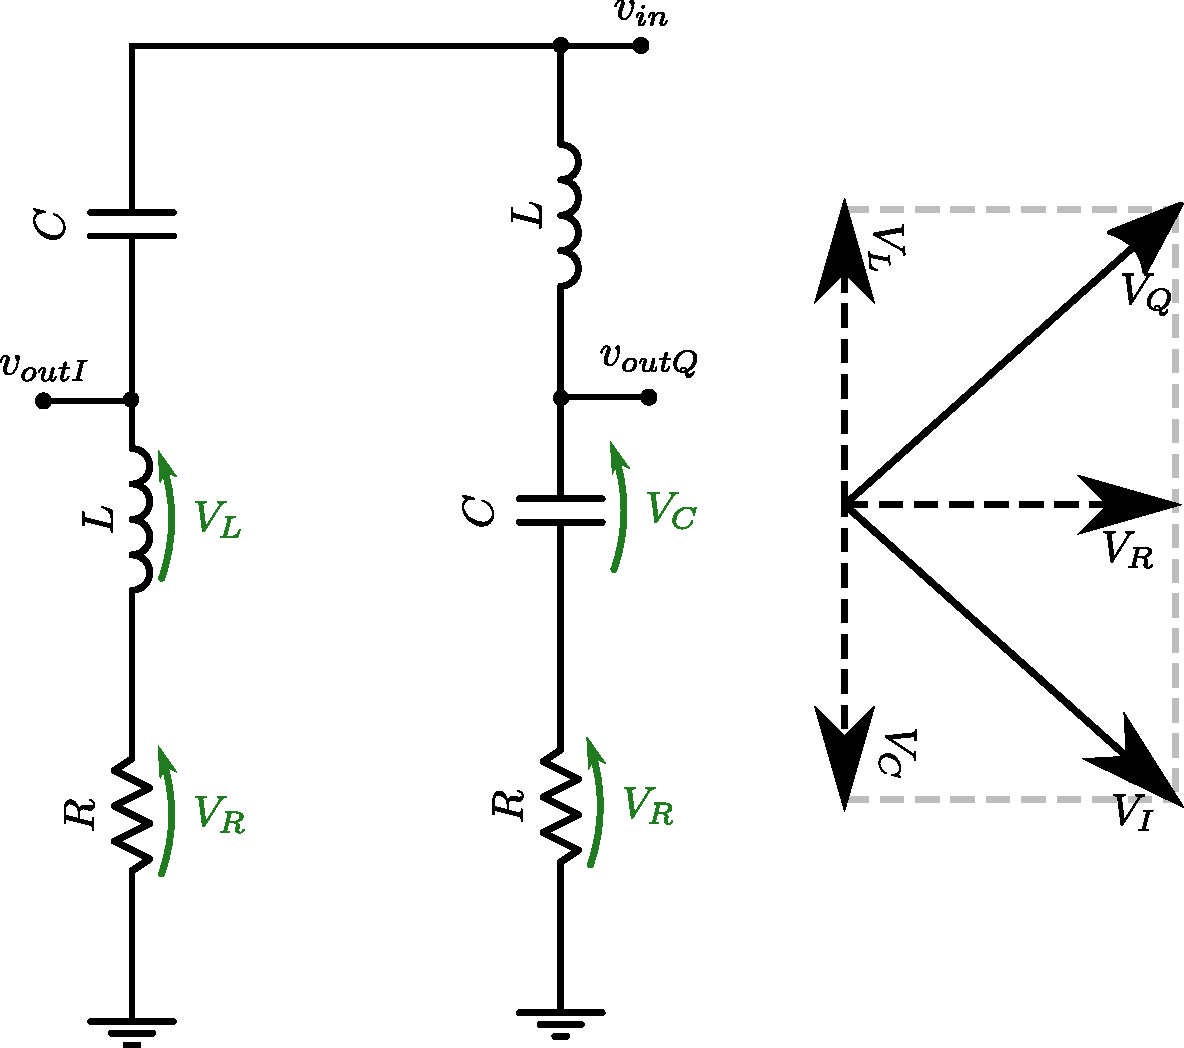
\includegraphics[width=0.8\linewidth]{qaf_single_ended.pdf}
  \caption{QAF single ended}
  \label{fig:qaf_single_ended}
\end{figure}


\begin{figure}[!htbp]
  \centering
  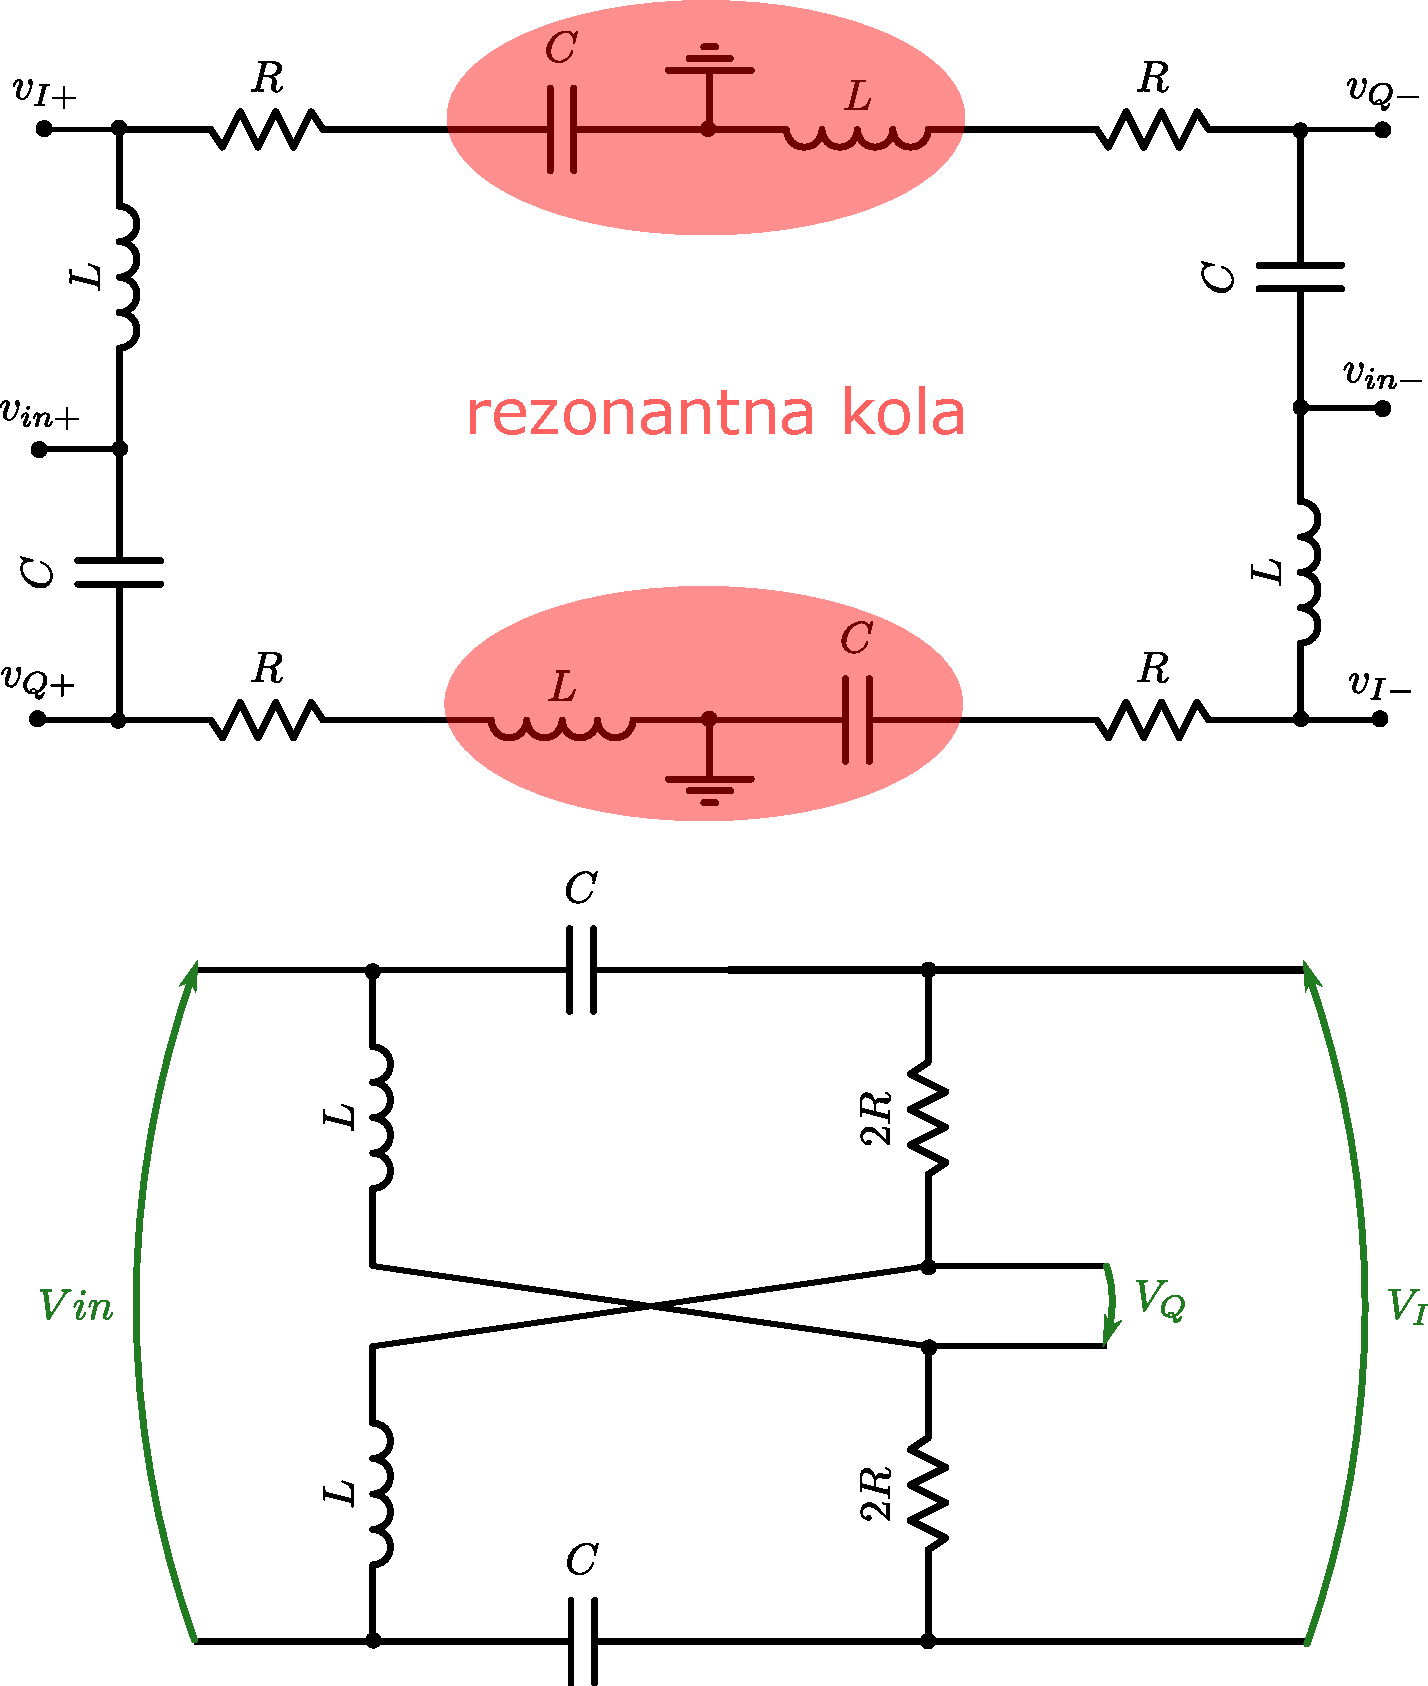
\includegraphics[width=\linewidth]{qaf_diff.pdf}
  \caption{Transformacija u diferencijalnu \textit{all-pass} mrežu}
  \label{fig:qaf_diff}
\end{figure}

Kao i RC-CR filtar, ni QAF nije imun na opterećivanje izlaza kapacitvnošću i zbog toga se koristi diferencijalni QAF. Izvođenje diferencijalnog kola iz kvadraturnog \textit{all-pass} filtra je prikazano na slici ~\ref{fig:qaf_diff}. Iskorišćena je sloboda u biranju vrednosti redno vezanih kondenzatora i kalema, pa su izabrane one najpogodnije, kada su u rezonanci, što znači da se mogu i izbaciti iz kola, što nam olakšava dizajn.

Razlika faza I i Q signala QAF-a odgovara geometriji nula u I/Q karakteristici:


\[
\begin{bmatrix}
    V_{I\pm}      \\
    V_{Q\pm}    
\end{bmatrix}   
=
V_{in} \times
\begin{bmatrix}
    \pm \dfrac{s^2 + \dfrac{2 \omega_{o}}{Q} s - \omega_{o}^2}{s^2 + \dfrac{2\omega_{o}}{Q} s - \omega_{o}^2} \\
    \mp \dfrac{s^2 - \dfrac{2 \omega_{o}}{Q} s - \omega_{o}^2}{s^2 + \dfrac{2\omega_{o}}{Q} s - \omega_{o}^2}
\end{bmatrix}
\]

\subsection{Diferencijalni degenerisani QAF}

Implementiranje generatora signala postaje teže na višim učestanostima, jer se po pravilu sadrže elemenate manjih kapacitivnosti i induktivnosti pa paraziti više dolaze do izražaja. Kod promene pojačanja pojačavača menjaju se paraziti, zbog toga se koristi diferecijalni generator, jer se i kontrola može napraviti diferencijalno ($I_{TOTAL}=I_{P}+I_{N}=const.$) pa generator vidi znatno manje promene impedanse na izlazu.

\begin{figure}[!htbp]
  \centering
  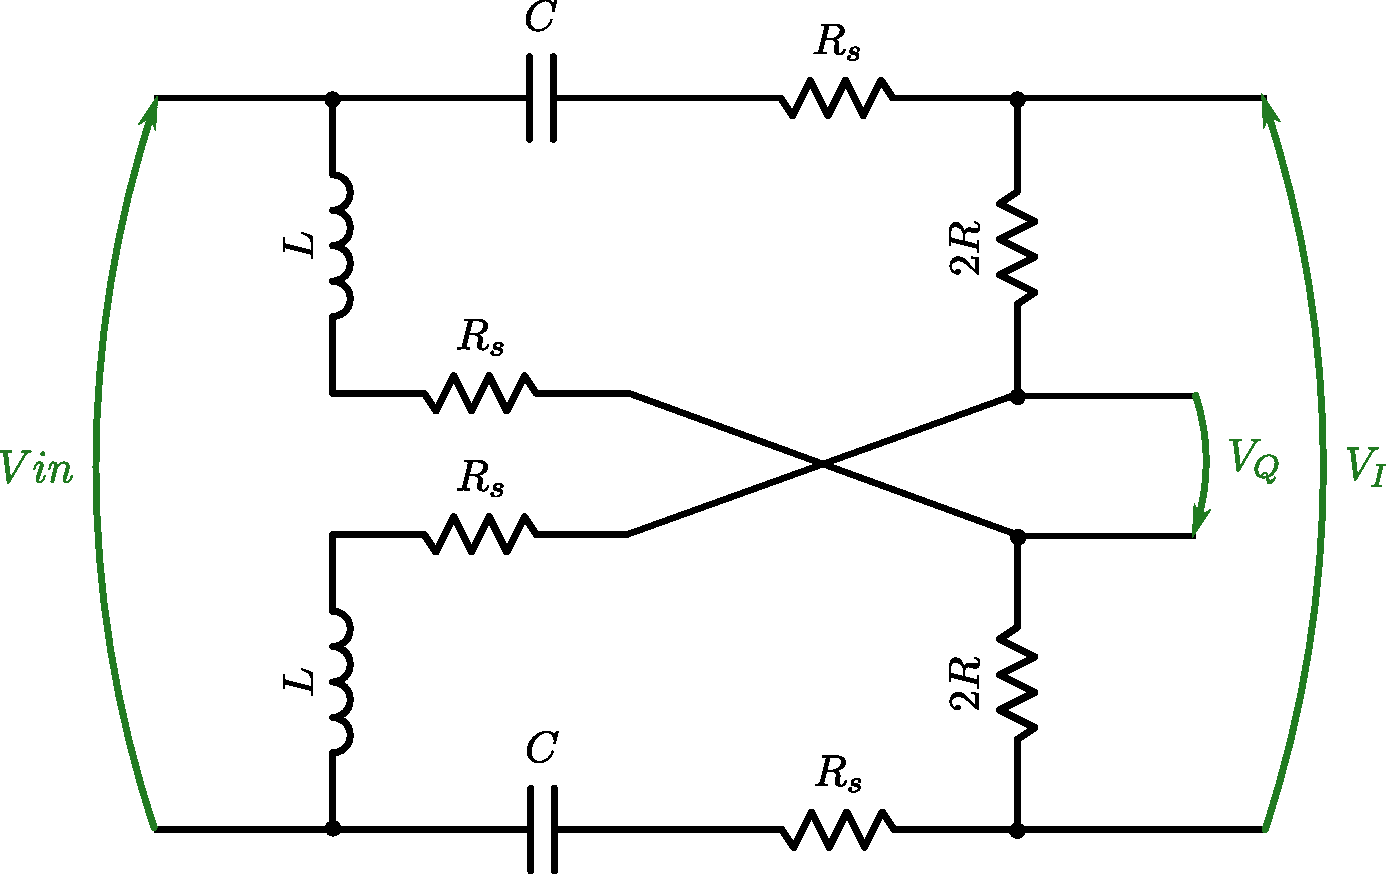
\includegraphics[width=\linewidth]{qaf_diff_degen.pdf}
  \caption{Degeneracija \textit{all-pass} mreže}
  \label{fig:qaf_diff_degen}
\end{figure}

Dodavanjem otpornosti na red sa reaktivnim elementima se smanjuje njihov faktor dobrote (Q) i povećava propusni opseg. Ali ove otpornosti povećavaju grešku amplitude, slabljenje I i Q signala i povećavaju potrošnju kola. Neke integrisane tehnologije poseduju otpornike u višim metalnim slojevima za pogoršavanje Q faktora pasivnih mreža za prilagođenje, ali IHP SiGe 130 nm tehnologija nema, pa se koriste parazitne otpornosti ili otpornici u nižim slojevima i supstratu.

Razlika faza I i Q signala degenerisanog QAF-a odgovara geometriji nula u I/Q prenosnoj karakteristici:

\[
\begin{bmatrix}
    V_{I\pm}      \\
    V_{Q\pm}    
\end{bmatrix}   
=
V_{in} \times
\begin{bmatrix}
    \pm \dfrac{s^2 + \dfrac{2\omega_{o}}{Q} s - \omega_{o}^2}{s^2 + \dfrac{2\omega_{o}}{Q}(1+\dfrac{R_s}{R}) s - \omega_{o}^2} \\
    \mp \dfrac{s^2 - \dfrac{2\omega_{o}}{Q} s - \omega_{o}^2}{s^2 + \dfrac{2\omega_{o}}{Q}(1+\dfrac{R_s}{R}) s - \omega_{o}^2}
\end{bmatrix}
\]

Prenosna karakteristika degenerisanog QAF-a ima iste nule kao i običan diferencijalni QAF, ali polovi se zbog pogoršanja Q faktora udaljavaju jedan od drugoga. \\

% Kao što se može videti na


\section{Vektor modulator}

Vektor modulator se sastoji od dva pojačavača linearno podesivog pojačanja (VGA - \textit{Variable Gain Amplifier}) napravljenih u topologiji Gilbertove ćelije. Diferencijalni I/Q izlazni signali QAF generatora pogone ova dva pojačavača (vidi sliku ~\ref{fig:vga_vmod}).

\begin{figure}[!htbp]
  \centering
  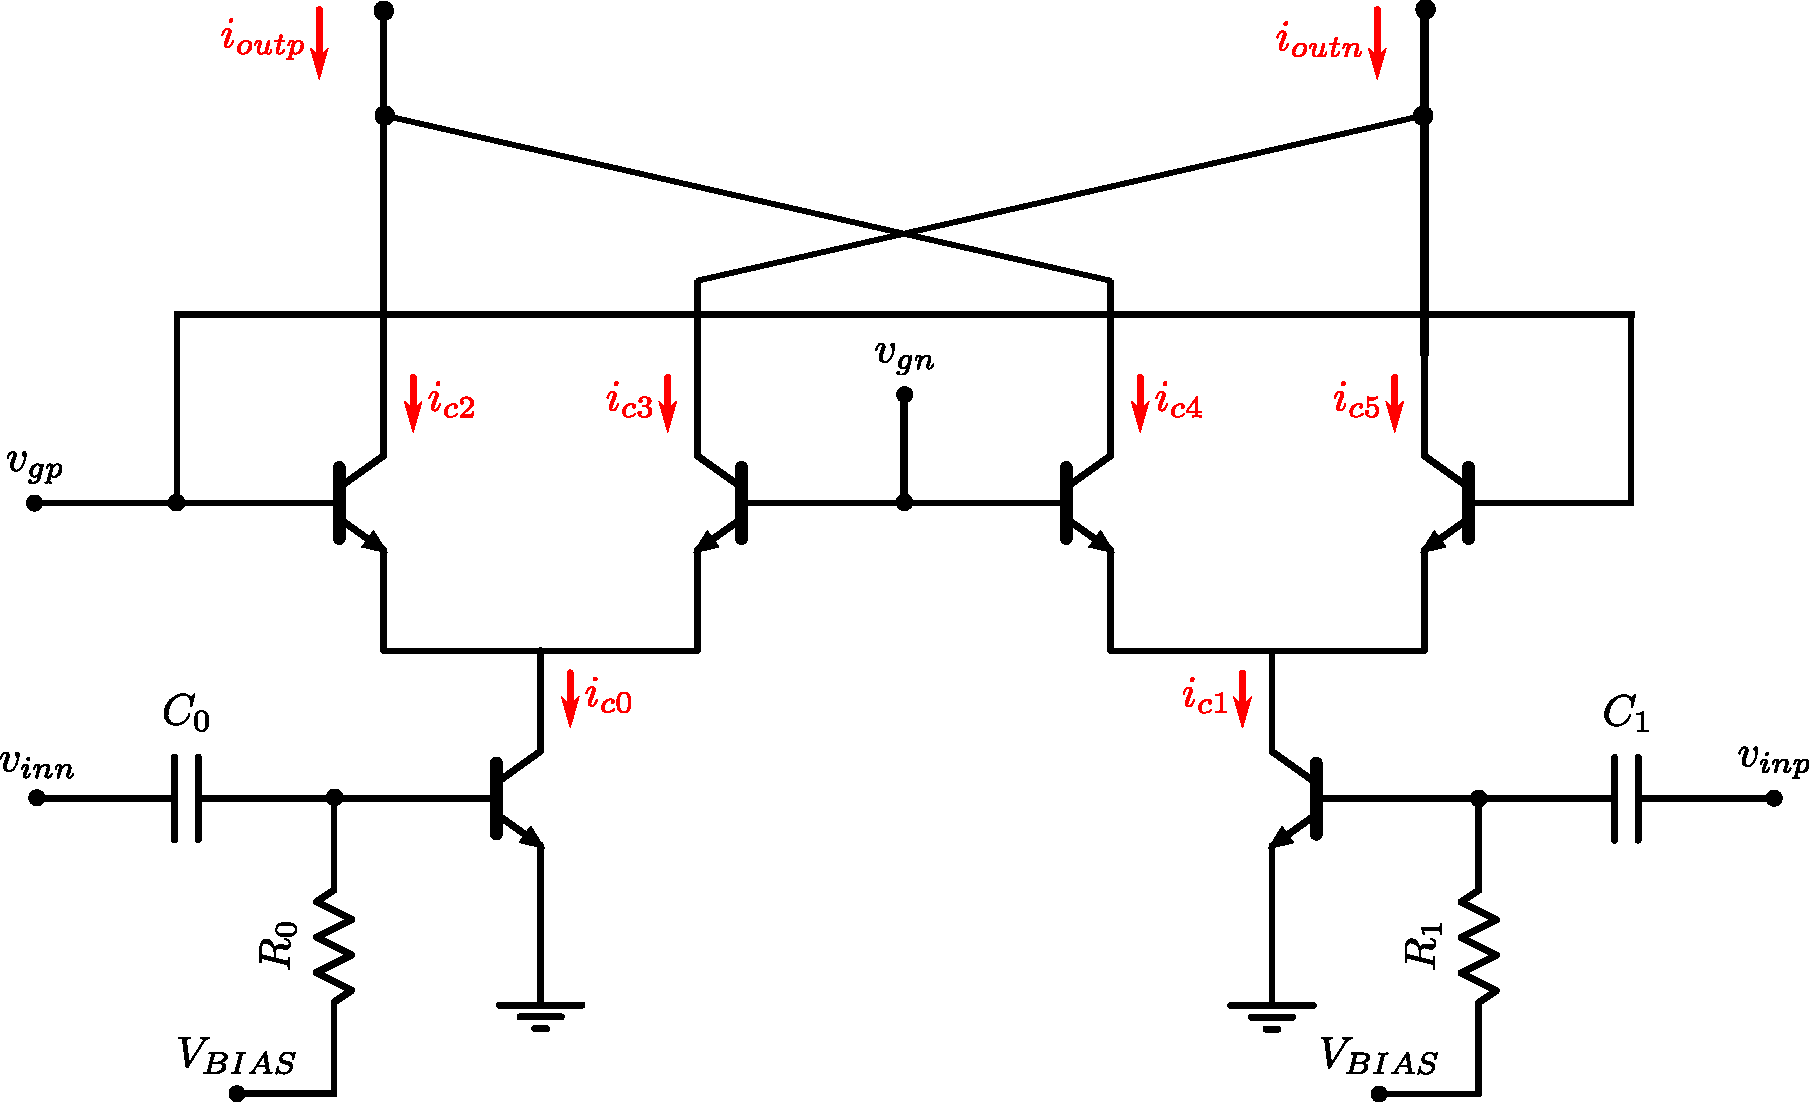
\includegraphics[width=\linewidth]{vga_vmod.pdf}
  \caption{Linearno podesiv pojačavač (Gilbertova ćelija)}
  \label{fig:vga_vmod}
\end{figure}


\begin{figure}[!htbp]
  \centering
  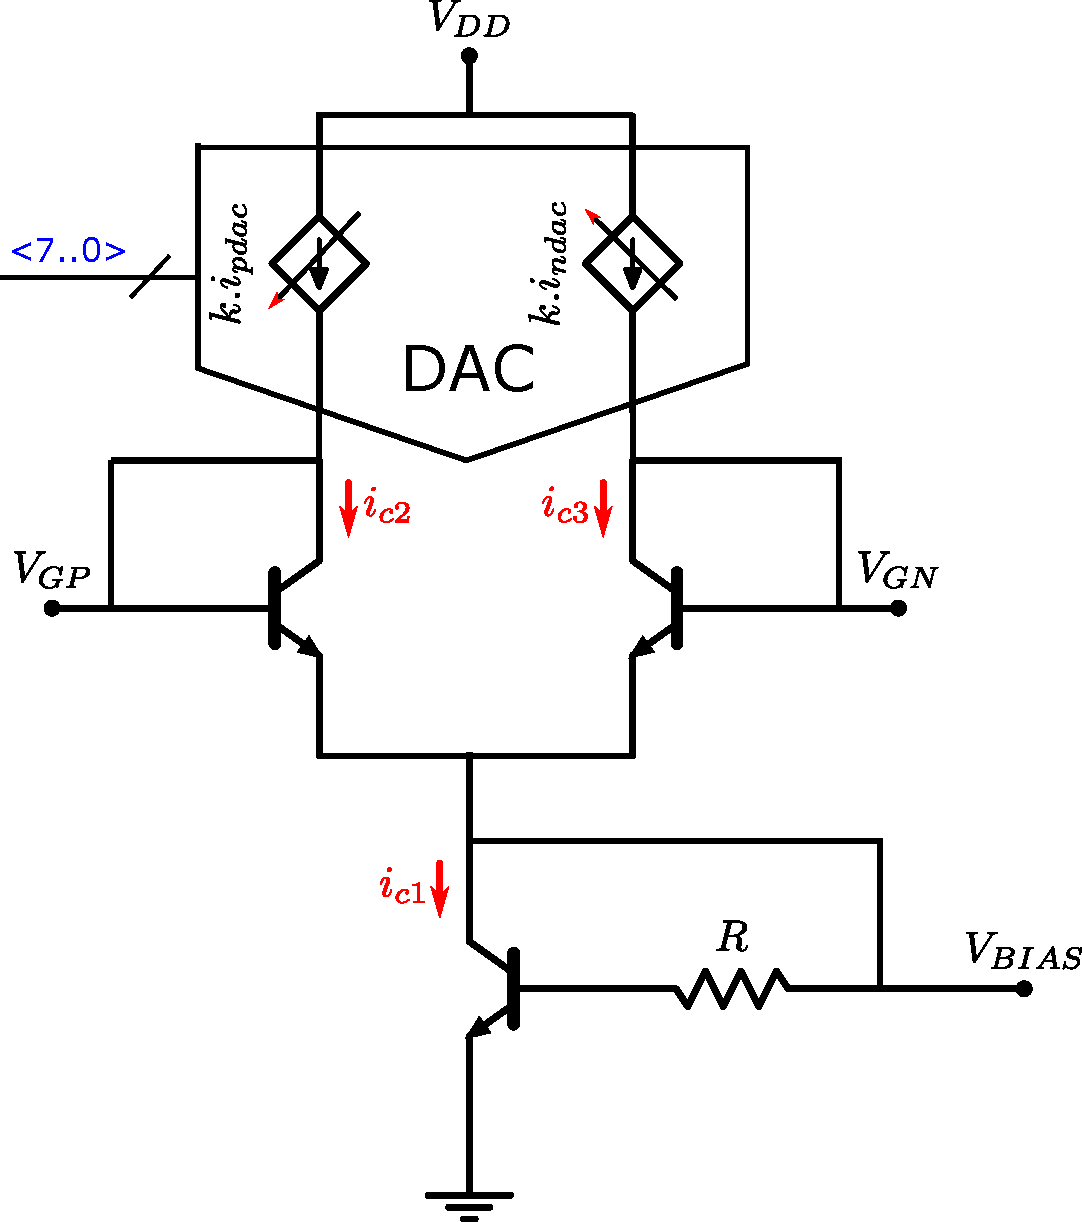
\includegraphics[width=\linewidth]{vga_bias.pdf}
  \caption{Kolo za polarizaciju \textit{VGA}}
  \label{fig:vga_bias}
\end{figure}

Linearnost zavisnosti pojačanja u odnosu na struju preslikavanja se može pokazati pomoću izvođenja.

Upotrebom Kirhofovog zakona za izlazne struje kolektora tranzistora ($Q_{1-4}$) se dobija:

\begin{align}
  \label{eqn:kcl}
  \begin{split}
   i_{outn} = i_{c5} + i_{c3}, \,
   i_{outp} = i_{c4} + i_{c2} \\
   i_{c0} = i_{c2} + i_{c3}, \, \, \, \,
   i_{c1} = i_{c4} + i_{c5} 
  \end{split}
\end{align}

a preslikavanjem struja:

\begin{align}
  \label{eqn:mirror}
  \begin{split}
     i_{c0} = i_{in}, \,
     i_{c1} = -i_{in}
  \end{split}
\end{align}

Transkonduktansa HBT bipolarnog tranzistora je proporcionalna struji kolektora:

\begin{equation}
  \label{eqn:transconductance}
  g_{m} = \dfrac{qI_c}{kT}
\end{equation}

pa se struje kolektora mogu izraziti preko odnosa transkonduktansnog pojačavača:

\begin{equation}
  \label{eqn:current_ratio}
  \dfrac{i_1}{i_2} = \dfrac{g_{m1}}{g_{m2}}
\end{equation}

Transkonduktanse tranzistora $Q2$ i $Q4$ su jednake kao i $Q3$ i $Q5$

\begin{align}
  \label{eqn:gm_equal}
  \begin{split}
     g_{m2} = g_{m5}, \,
     g_{m3} = g_{m4}
  \end{split}
\end{align}


Koristeći jednačine~\eqref{eqn:kcl},~\eqref{eqn:mirror},~\eqref{eqn:transconductance} i~\eqref{eqn:current_ratio}, struje $i_{c2-5}$ se mogu izraziti:

\begin{align}
  \label{eqn:deriv2}
  \begin{split}
    \dfrac{i_{c2}}{i_{in}} = \dfrac{i_{c2}}{i_{c2} + i_{c3}} = \dfrac{g_{m2}}{g_{m2} + g_{m3}}, \\
    -\dfrac{i_{c5}}{i_{in}} = -\dfrac{i_{c5}}{i_{c4} + i_{c5}} = -\dfrac{g_{m5}}{g_{m4} + g_{m5}} \\
  \end{split}
\end{align}

Na osnovu ~\eqref{eqn:gm_equal} i dualnosti parova struja kolektora, struje $i_{c2-5}$ se mogu izraziti kao:

\begin{align}
  \label{eqn:deriv3}
  \begin{split}
    i_{c2} = -i_{c5} = \dfrac{g_{m2}}{g_{m2} + g_{m3}} i_{in} = \dfrac{I_{c2}}{I_{c2} + I_{c3}} i_{in}, \\
    i_{c3} = -i_{c4} = \dfrac{g_{m3}}{g_{m2} + g_{m3}} i_{in} = \dfrac{I_{c3}}{I_{c2} + I_{c3}} i_{in}, \\
  \end{split}
\end{align}

\begin{equation*}
  \label{eqn:out_current}
    i_{outp} = - i_{outn} 
\end{equation*}


\begin{equation*}
  \label{eqn:out_current}
    i_{outp} = i_{c2} + i_{c4} = \dfrac{I_{c2} - I_{c3}}{I_{c2} + I_{c3}}i_{in} = \dfrac{I_{PDAC} - I_{NDAC}}{I_{PDAC} + I_{NDAC}}i_{in} 
\end{equation*}


Poželjno je da $I_{PDAC} + I_{NDAC} = const.$ kako bi generator I/Q signala video manje više konstantu impedansu na svom izlazu, pa od promenljivih na izlazu nam ostaje samo razlika $I_{PDAC} - I_{NDAC}$. Osmobitni DA konvertor nam daje kontrolu struje $N * I_{REF\_DAC}$, gde se N nalazi u opsegu od -127 do 126.(127?)

\begin{equation}
  \label{eqn:gm_out}
    g_{moutp} = \dfrac{N*I_{REF}}{I_{DAC}} g_{min}
\end{equation}

Sve ovo važi i za I i Q deo vektor-modulatora:

\begin{align}
  \label{eqn:gm_IQ}
  \begin{split}
    g_{moutp\_I} = \dfrac{N_I*I_{REF\_I}}{I_{DAC\_I}} g_{min\_I} \\
    g_{moutp\_Q} = \dfrac{N_Q*I_{REF\_Q}}{I_{DAC\_Q}} g_{min\_Q} \\
  \end{split}
\end{align}

% Faza izlaza se linearno kontroliše i može se odrediti kao nula prenosne karakteristike VGA?

% TODO: Prenosna karakteristika VGA

\begin{equation}
  \label{eqn:out_phase}
  \theta = tan^{-1}(\dfrac{N_{Q}}{N_{I}})
\end{equation}


\begin{figure}[!htbp]
  \centering
  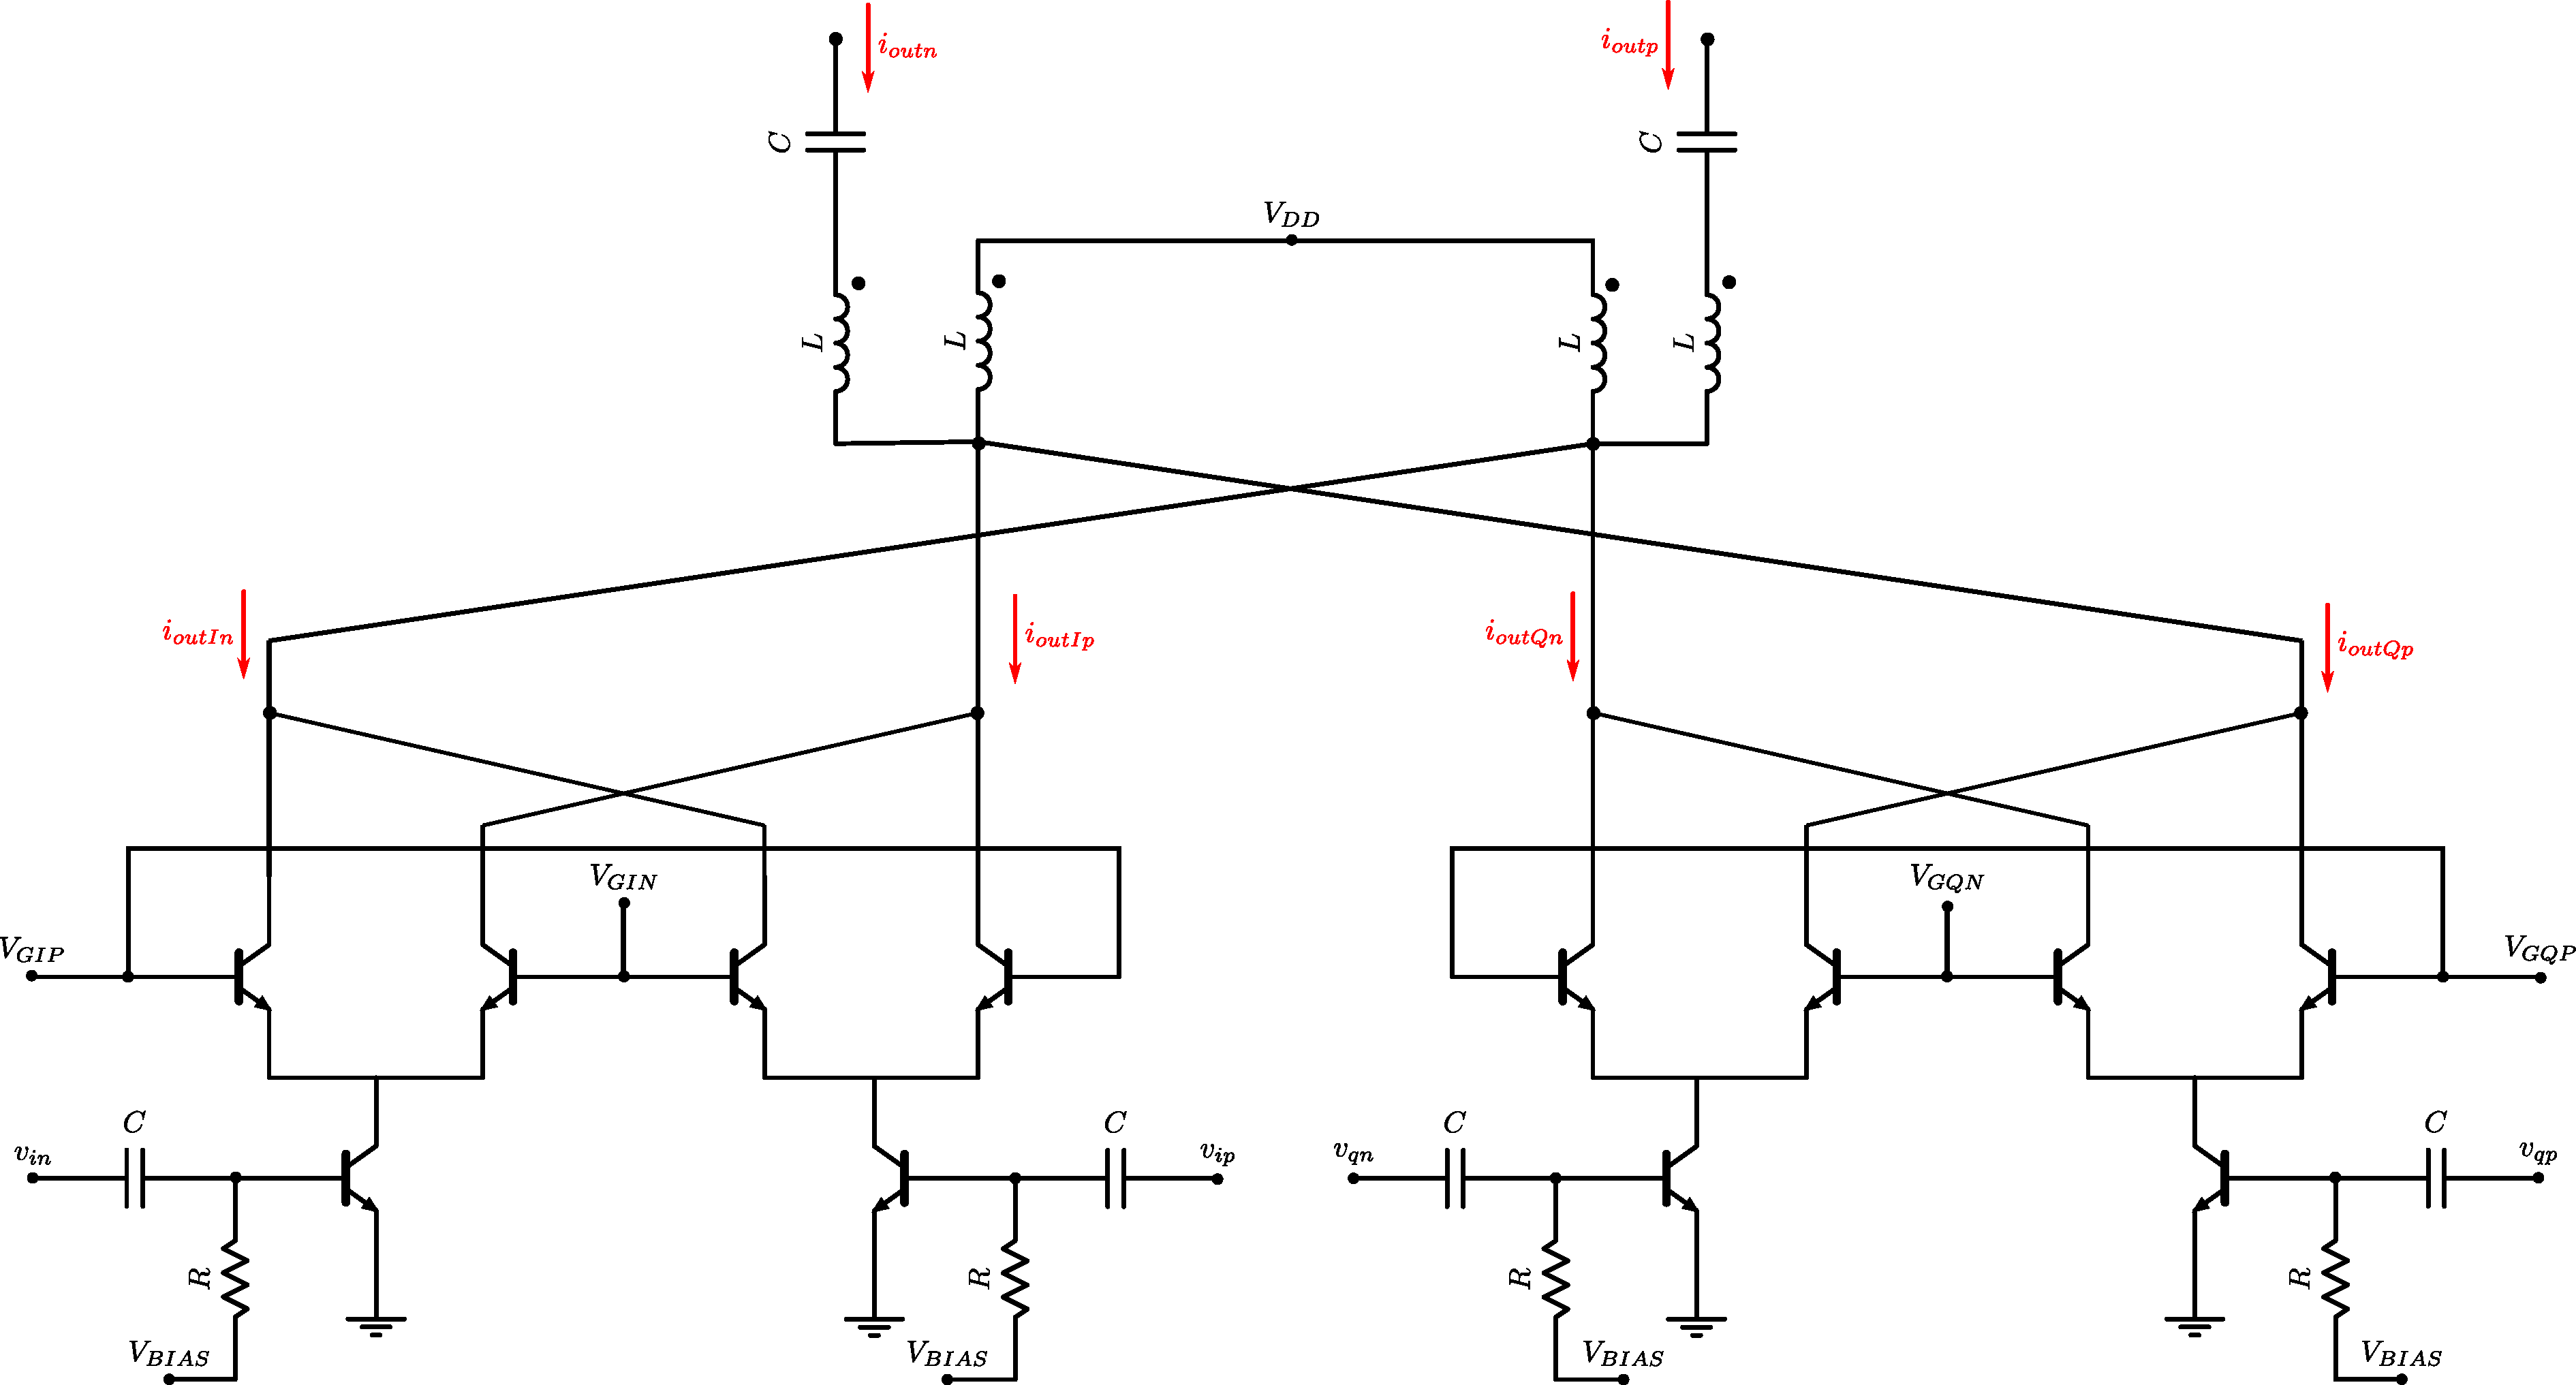
\includegraphics[width=\linewidth]{vmod.pdf}
  \caption{Vektor modulator}
  \label{fig:vmod}
\end{figure}


% Eqn.~\eqref{eqn:eqlabel} has a single label split
% across the two equations, as you can see here:
% \begin{align}
% \label{eqn:eqlabel}
% \begin{split}
%  f(x) &= x^2 ,
% \\
%  g(x) &= \exp( x ) .
% \end{split}
% \end{align}

Za kaleme u kombajneru je bitno da imaju što bolji Q faktor kako bi pojačanje \textit{VGA} bilo što veće!


\subsection{Kolo za polarizaciju modulatora}

Linearna kontrola Gilbertove ćelije zasnovane na MOS tranzistorima je teško ostvariva jer nelinearna zavisnost pojačanja od kontrole struje zahteva kompleksnu višebitnu kontrolu. \\

Upravljanje pojačanjem konfigurablinih pojačavača se vrši polarizacijom bipolarnih tranzistora Gilbertovih ćelija preslikavanjem struja $I_{PDAC}$ i  $I_{NDAC}$ za I i Q signale nezavisno. \\

% TODO: Izračunaj promenu pojačanja po promeni analogne* kontrole?


\section{Digitalno-analogna kontrola modulatora}

% Bitne specifikacije DAK-a !

Preslikana struja se generiše DA konvertorom. DA konvertor je projektovan na osnovu kombinacije R-2R lestvičaste arhitekture za niže bitove i termometarskog koda u kome se izražavaju najviša 3 bita. Deo arhitekture zasnovan na R-2R lestvicama zahteva više otpornika, ali zauzima manje prostora zbog manjeg broja tranzistora, dok arhitektrura sa termometarskim kodiranjem nam daje preciznije balansiranje na izlazu na štetu veće površine digitalno analogne kontrole na čipu. Na ovaj način se u zavisnosti od potreba za površinom i performansama, može odrediti koliko će bitova pripadati kojoj arhitekturi. \\

% \begin{table}[!htbp]
%   \begin{center}
%     \begin{tabular}{| c | c | c |}
%       \hline
%       Arhitektura & R-2R & Izabrana  \\
%       \hline
%       termometarski kod & & \\
%       \Xhline{2\arrayrulewidth}
%       otpornici & & \\
%       \hline
%       prekidači & & \\
%       \hline
%       gejtovi & & \\
%       \hline
%     \end{tabular}
%   \end{center}
%   \caption{Arhitekture digitalno analogne kontrole}
% \end{table}






% Korišćena je statička digitalno-analogna kontrola.

\begin{figure}[!htbp]
  \centering
  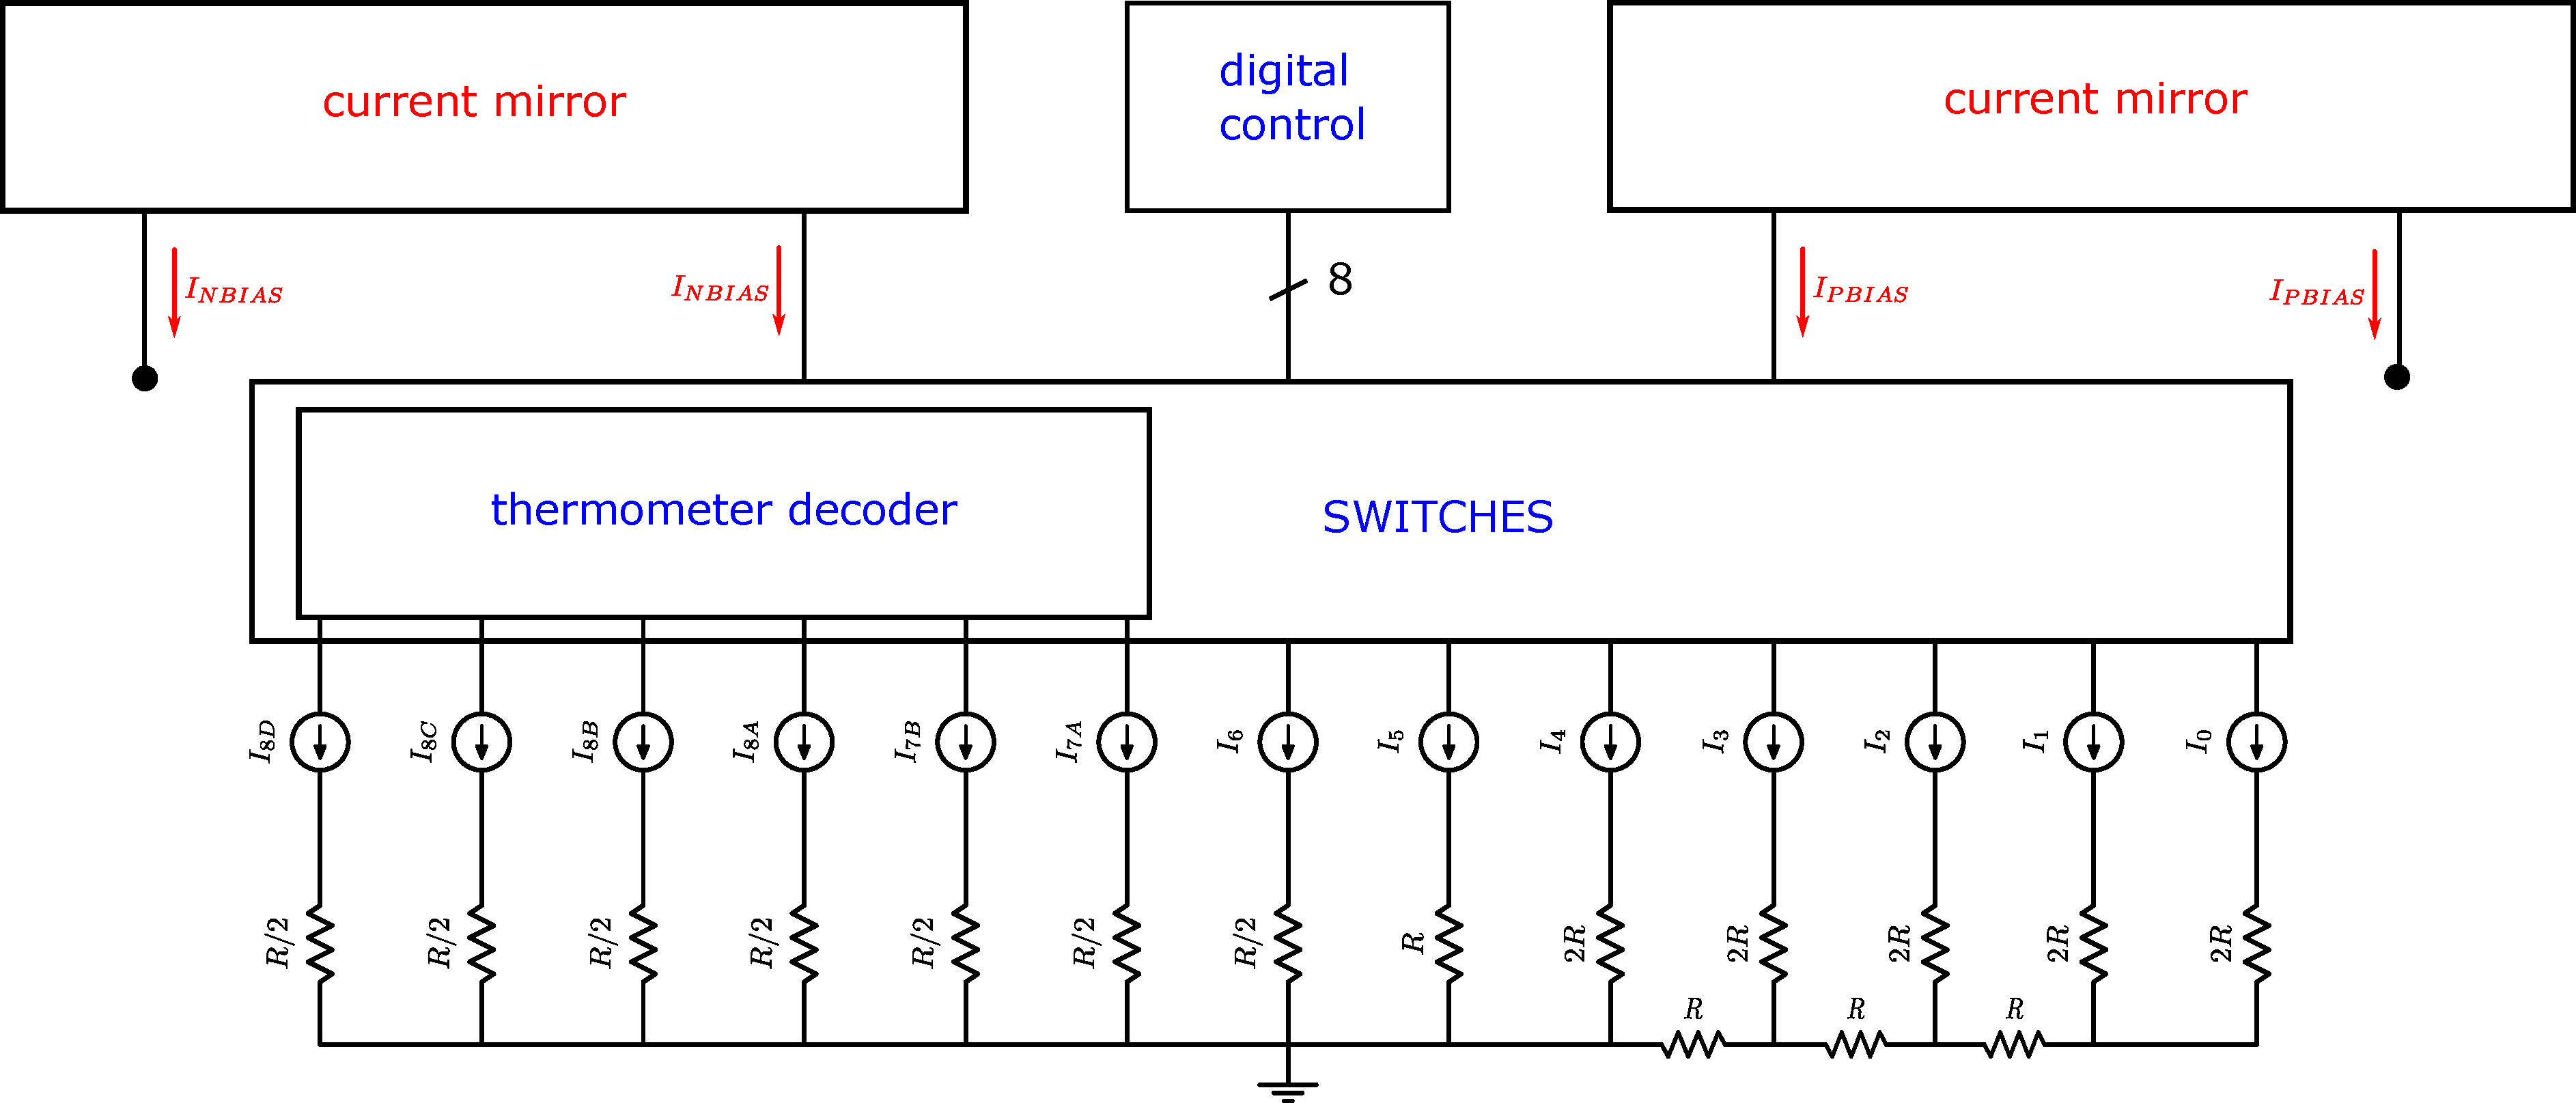
\includegraphics[width=\linewidth]{dac_core.pdf}
  \caption{Arhitektura digitalno analogne kontrole}
  \label{fig:dac_core}
\end{figure}

\subsection{Strujno ogledalo}

Strujno ogledalo pruža potrebno preslikavanje struje generisane DA konvertorom u struju kojom se polariše VGA održavajući linearnost nezavisno od ulaznih kontrolnih bitova. Kako bi se ovo postiglo potrebno je da naponi drejna budu konstantni na tranzistorima reference i ogledala. \\

\subsection{Stabilnost strujnog ogledala}

Strujno ogledalo osciluje kada se pomoću Verilog-A bloka generišu njegovi signali za digitalnu kontrolu kao inkrement na nekoj učestanosti. Posle nekoliko promena digitalne kotrole struja proosciluje (kao kod \cite{zeki07} Fig. 10a). Zamenom ovog strujnog ogledala za obično kaskodno problemi nestaju.

\begin{figure}[!htbp]
  \centering
  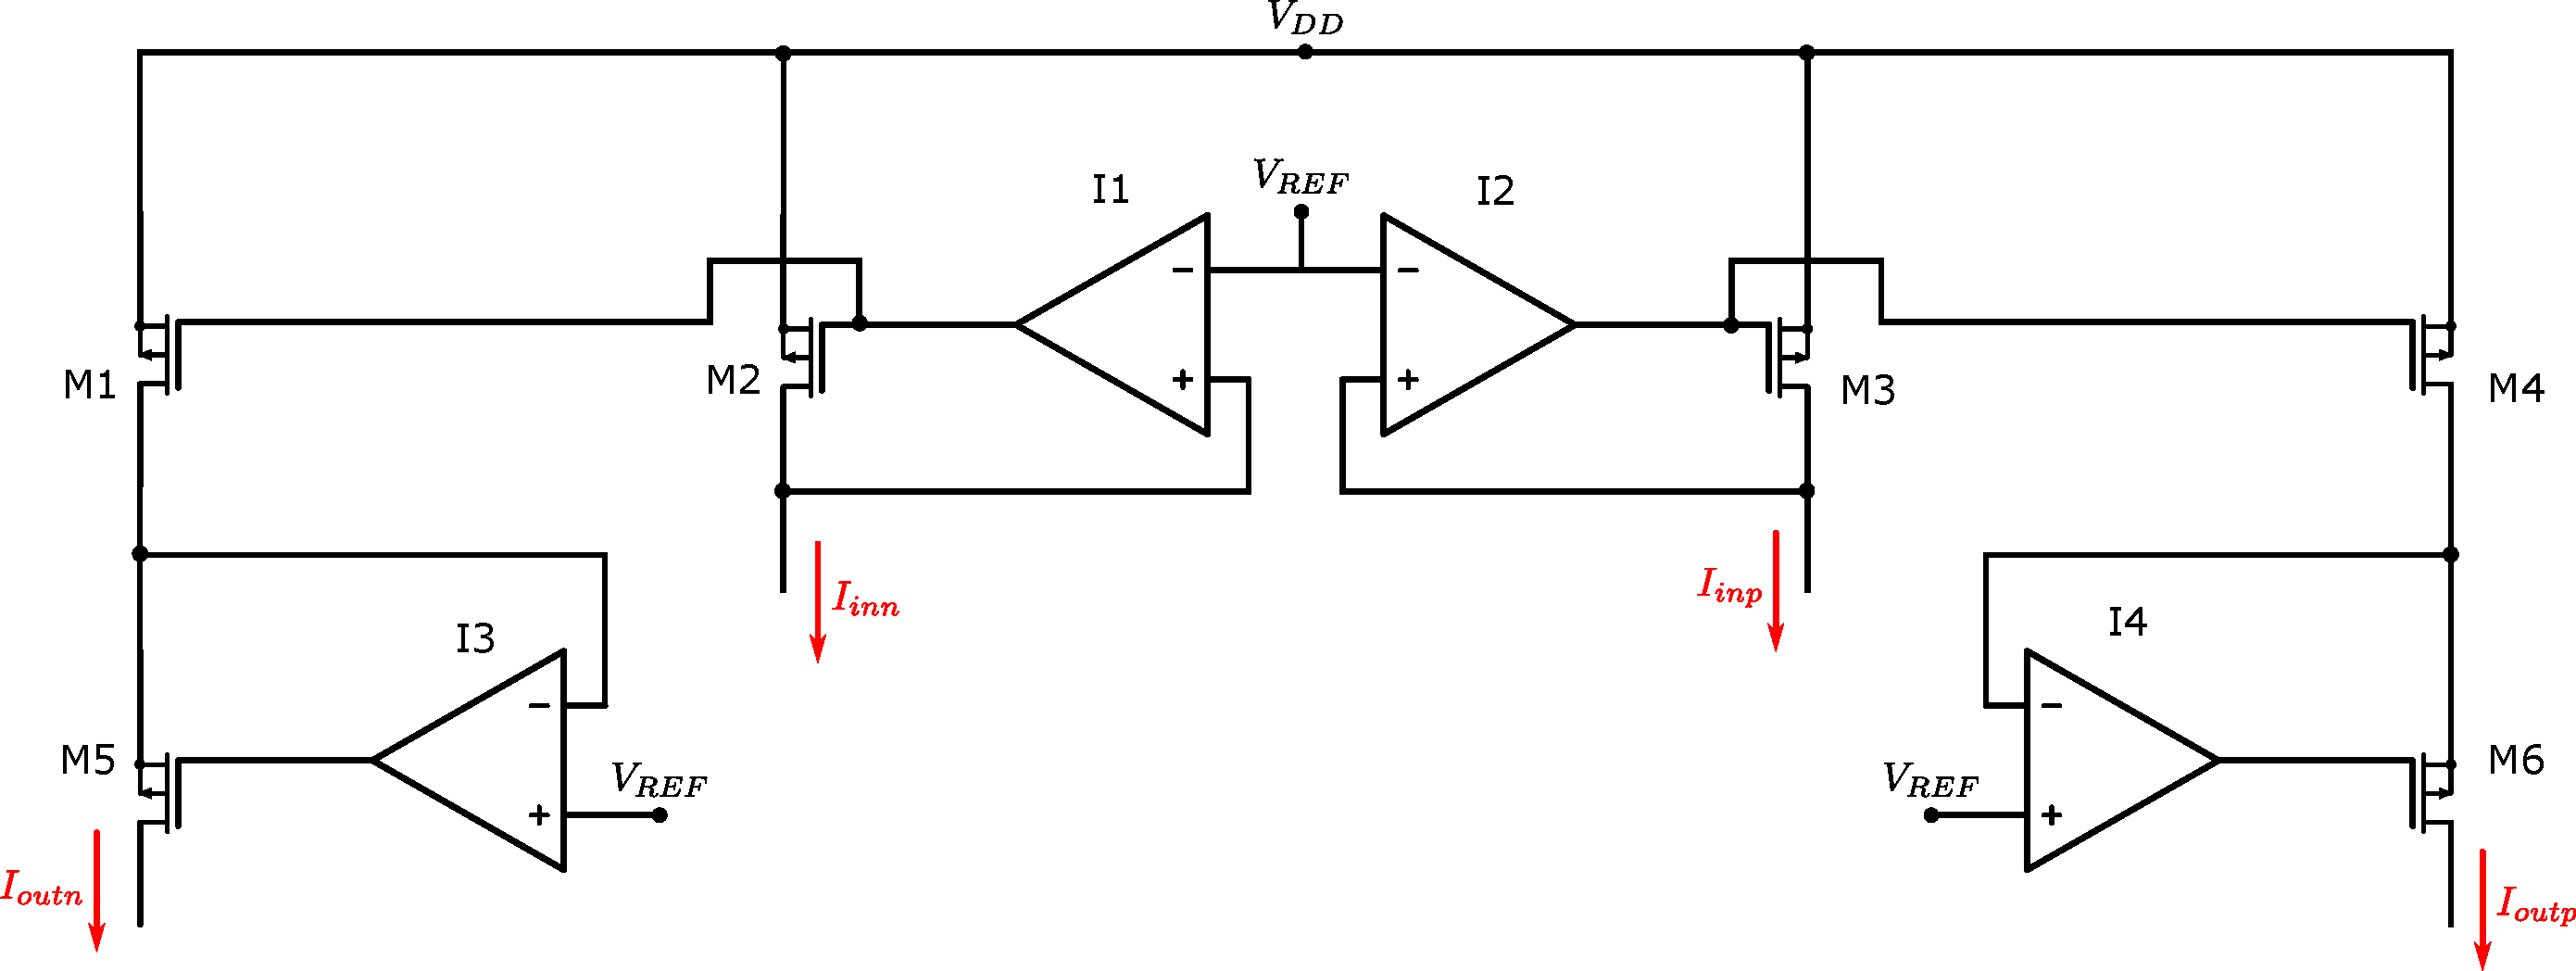
\includegraphics[width=\linewidth]{mirror_detail.pdf}
  \caption{Šema strujnog ogledalo}
  \label{fig:mirror_detail}
\end{figure}


\begin{figure}[!htbp]
  \centering
  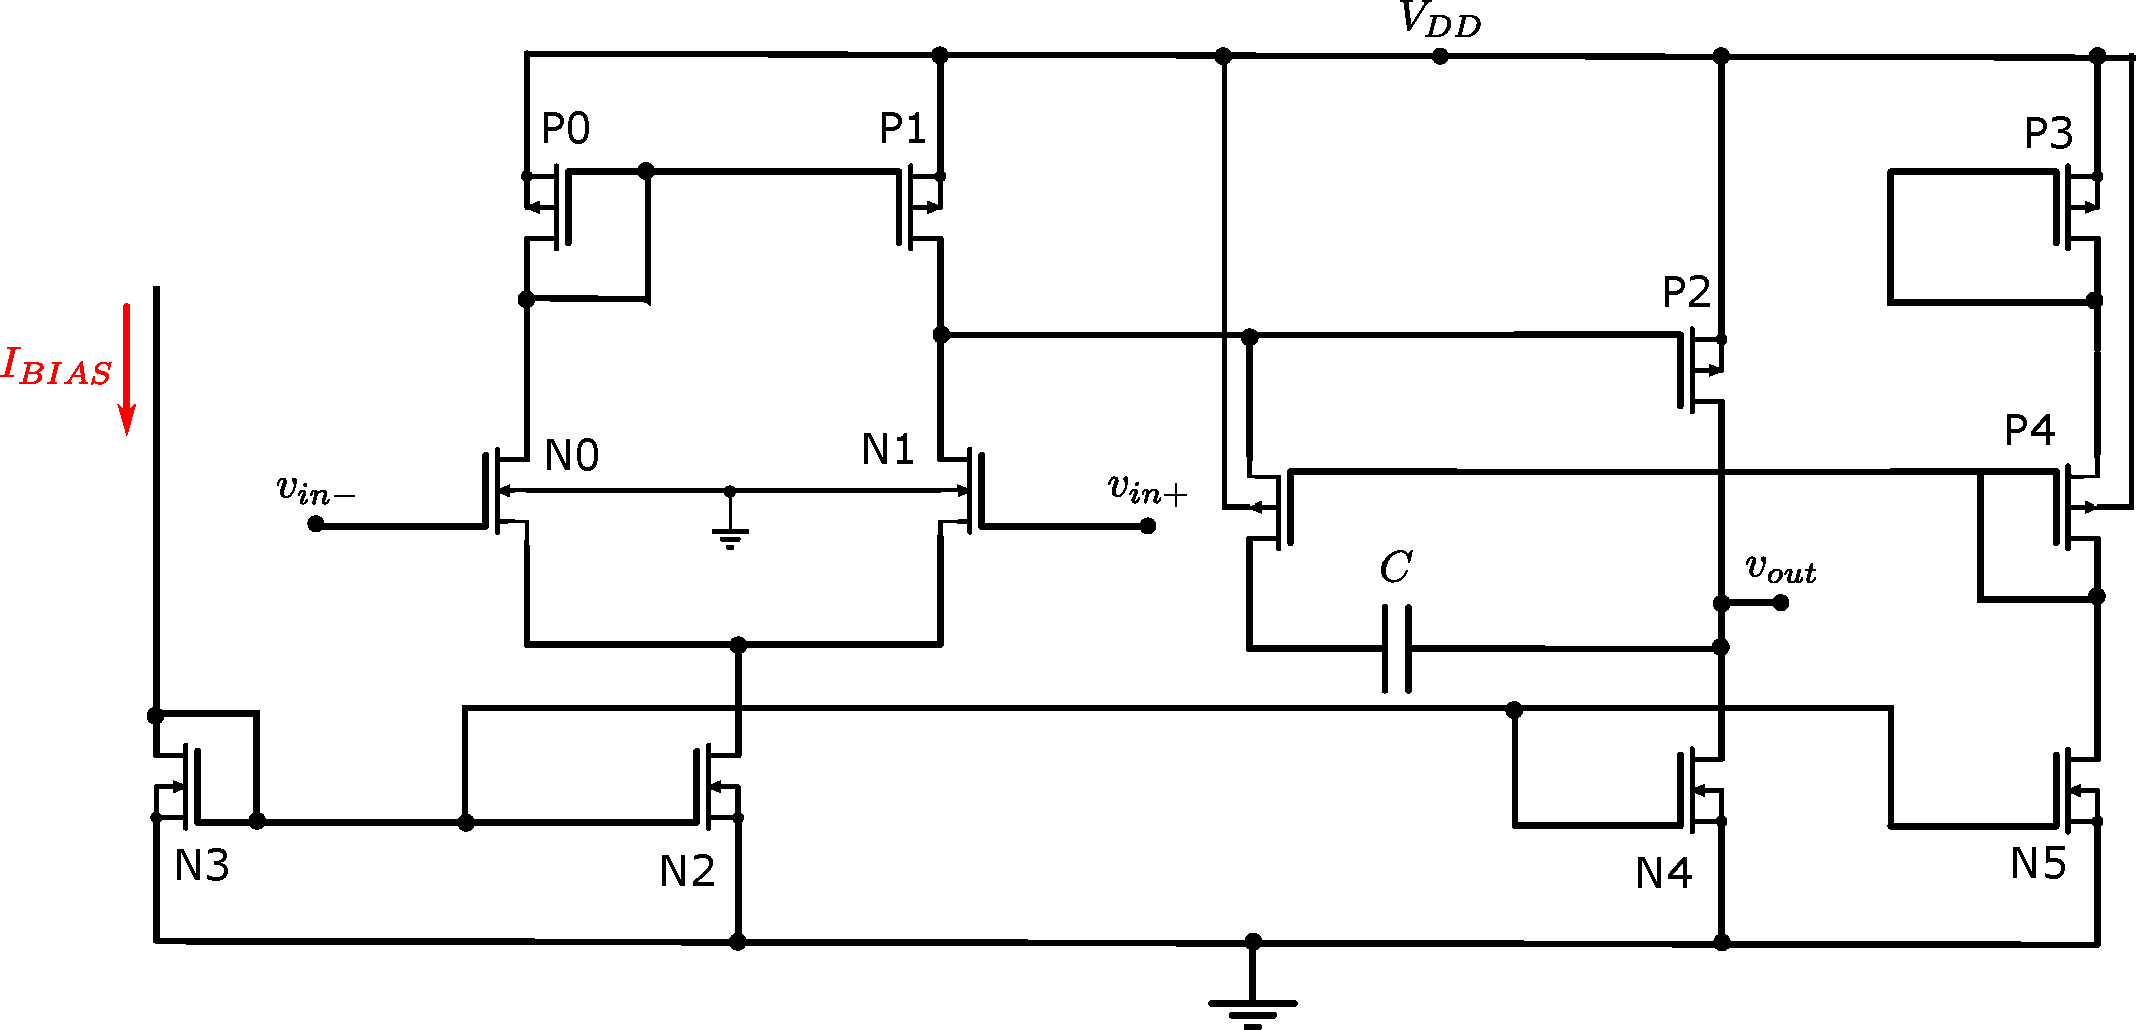
\includegraphics[width=\linewidth]{servo_oa.pdf}
  \caption{Servo operacioni pojačavač}
  \label{fig:servo_oa}
\end{figure}

\section{Množenje učestanasti}

Veoma važna specifikacija faznog pomerača je opseg kontrole, i za mnoge primene je neophodan opseg od $360^o$. Treba uzeti i obzir mogućnost umnožavanja ostvarene fazne kontrole. Po pravilu ovaj metod bi trebalo da relaksira zahteve za faznu kontrolu i varijaciju amplitude, ali poveća potrošnju jer ovi množači učestanosti moraju biti malošumni i linearni kako ne bi došlo do degradacije signala. \cite{ellinger10}

% Phase Control Range/
% Frequency Multiplication
% One important design parameter for phase shifters is
% the phase control range. For many applications a phase
% control range of 360° is required. However, the phase
% control range has to be traded off with other param-
% eters, which makes the design challenging. Is it pos-
% sible to multiply the phase control range in a relatively
% simple way?
% Consider that frequency multiplication divides the
% signal period duration. Consequently, the phase con-
% trol range is multiplied by the factor of the frequency
% multiplication. Typically, the method of frequency/
% phase multiplication relaxes the contradicting con-
% straints regarding the phase control range and ampli-
% tude variations. The drawback is the additional power
% consumed by the frequency multipliers [38], which
% should have good linearity and low noise to avoid sig-
% nal deteriorations.

\section{Blokovi pomerača faze}

% Podeli u core blokove i momentum blokove ... 
% Izbaci potrošnju 

\begin{center}
  \begin{tabular}{| c | c | c |}
    \hline
    blok & podblok & tip bloka/podbloka \\
    \Xhline{2\arrayrulewidth}
    vmod\_dac & / & schematic \\
    \hline
    vmod\_dac & core & = \\ 
    \hline
    vmod\_dac & bias & = \\
    \hline
    vmod\_dac  & mirror & = \\
    \hline
    vmod\_dac & oa\_servo\_3p3 & = \\
    \Xhline{2\arrayrulewidth}
    vmod\_balun & / & schematic \\
    \hline
    vmod\_balun & se2diff & ideal\_sch + sch \\
    \hline
    vmod\_balun & diffamp & ideal\_sch + sch \\
    \Xhline{2\arrayrulewidth}
    vmod\_qaf & / & momentum\\
    \hline
    vmod\_qaf & buffer & schematic\\
    \Xhline{2\arrayrulewidth}
    vmod\_vga &  / & schematic\\
    \hline
    vmod\_vga & bias & schematic \\
    \hline
    vmod\_vga & core & schematic \\
    \hline
    vmod\_vga & input_match & ideal\_sch \\
    \hline
    vmod\_vga & load & ideal\_sch \\
    \hline
  \end{tabular}
\end{center}



\section{Broj bitova pomerača faze}

Procena broja bitova rezolucije faznog pomeraja je ostvarena pomoću simulacija na centralnoj učestanosti od $28$ GHz, posmatranjem amplitude i faze izlaznog napona, pri promeni digitalne kontrole I i Q dela vektor modulatora. Pošto prolazak kroz ove dve 8-bitne kontrole je vremenski i resursno previše zahtevna za samo procenu rada ovog pomerača faze, pretraga je veštački smanjena, smanjivanjem bitova rada digitalne kontrole (svaki drugi, svaki četvrti ...). Dobijeni rezultati za fazu i amplitudu  za smanjeni broj kombinacija su korišćeni tako što su odabrane kombinacije sa približno istom amplitudom (pojačanjem). Radi jednostavnosti su izabrane vrednosti blizu srednje vrednosti (što se ne mora raditi, može i oko željenog pojačanja, optimizovane vrednosti tako daje najmanje odstupanje faza od idealnih). Izabrane kombinacije su uporođene sa raspodelom faze idealnog pomerača faze, i kao ocenu kvaliteta su uzeti odstupanja faze od idealne vrednosti najbliže odabrane kombinacije i uzeti parametar amplitudskog odstupanja za odabir samih kombinacija. \\

Ovaj postupak bi trebalo da bude vizuelno identičan kao iscrtavanje kruga na polarnom koordinatnom sistemu sa konstelacijom i određivanjem najbližih tačaka tom krugu na idealni diskretnim tačkama čiji broj odgovara. \\

Za dozvoljenu amplitudsku grešku od 0.5 dB i 6 bita tačnosti pomerača faze, koristeći degenerisane digitalno analogne kontrole gde se koristi svaka druga kombinacija (efektivno je 7-bitna DA kontrola), dobija se maksimalna fazna greška $1.29^o$ stepeni, a \textit{rms} greška $0.39^o$ stepeni.  \\

NAPOMENA: U prilogu pdf-a se nalazi i \textit{python} skripta koja je korišćena za procenu broja bitova. Ulazni podaci su dobijeni pomoću \textit{testbench}-a \textit{Cadence}-ovog simulatora u .csv formatu.

\section{Rezultati simulacija}

Pomerač faze (i QAF) se može okarakterisati i pomoću rms vrednosti odstupanja faze i pojačanja na željenom opsegu (slike~\ref{fig:gain_error_rms} i~\ref{fig:phase_error_rms}, gde se posmatra promena odstupanja u zavisnosti od razlike između struja za polarizacije, tj. $g_m$-a. ).
Na slikama~\ref{fig:gain_error} i~\ref{fig:phase_error} se mogu videti greške razlike faze i pojačanja signala u kvadraturi na opsezima učetanosti. Greška pojačanja je manja od $1 dB$, a greška razlike faze je manja od $25^o$. Pogoršavanjem Q faktora kalema i kondenzatora se može smanjiti greška faze na štetu slabljenja signala u kvadraturi.  
Ostvarena potpuna kontrola opsega faza je prikazana na slici~\ref{fig:phase_out_signal}, a linearna kotrola VGA na slici~\ref{fig:vga_linearity} za pun opseg digitalne kontrole VGA. \\

NAPOMENA:
Dati grafici su prikazani kao demonstracija ograničenja i mogućnosti tehnologije i topologije za neke kritične aspekte pomerača, i nisu simulirani za identične blokove, jer su oni ionako skloni promenama.


\begin{figure}[!htbp]
  \centering
  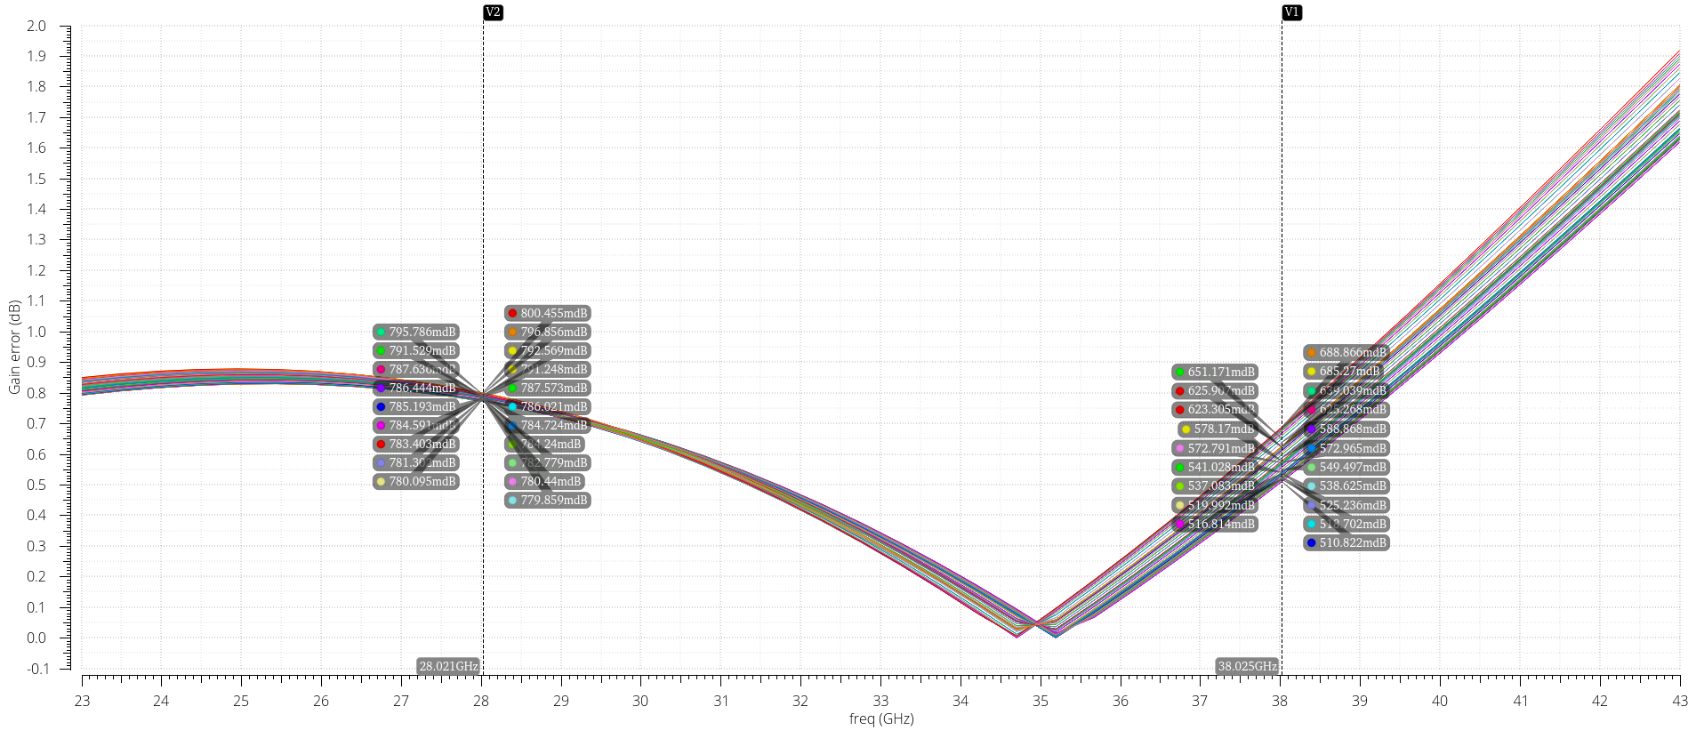
\includegraphics[width=\linewidth]{gain_error.png}
  \caption{Greška amplitude I/Q signala na opsegu učestanosti}
  \label{fig:gain_error}
\end{figure}

\begin{figure}[!htbp]
  \centering
  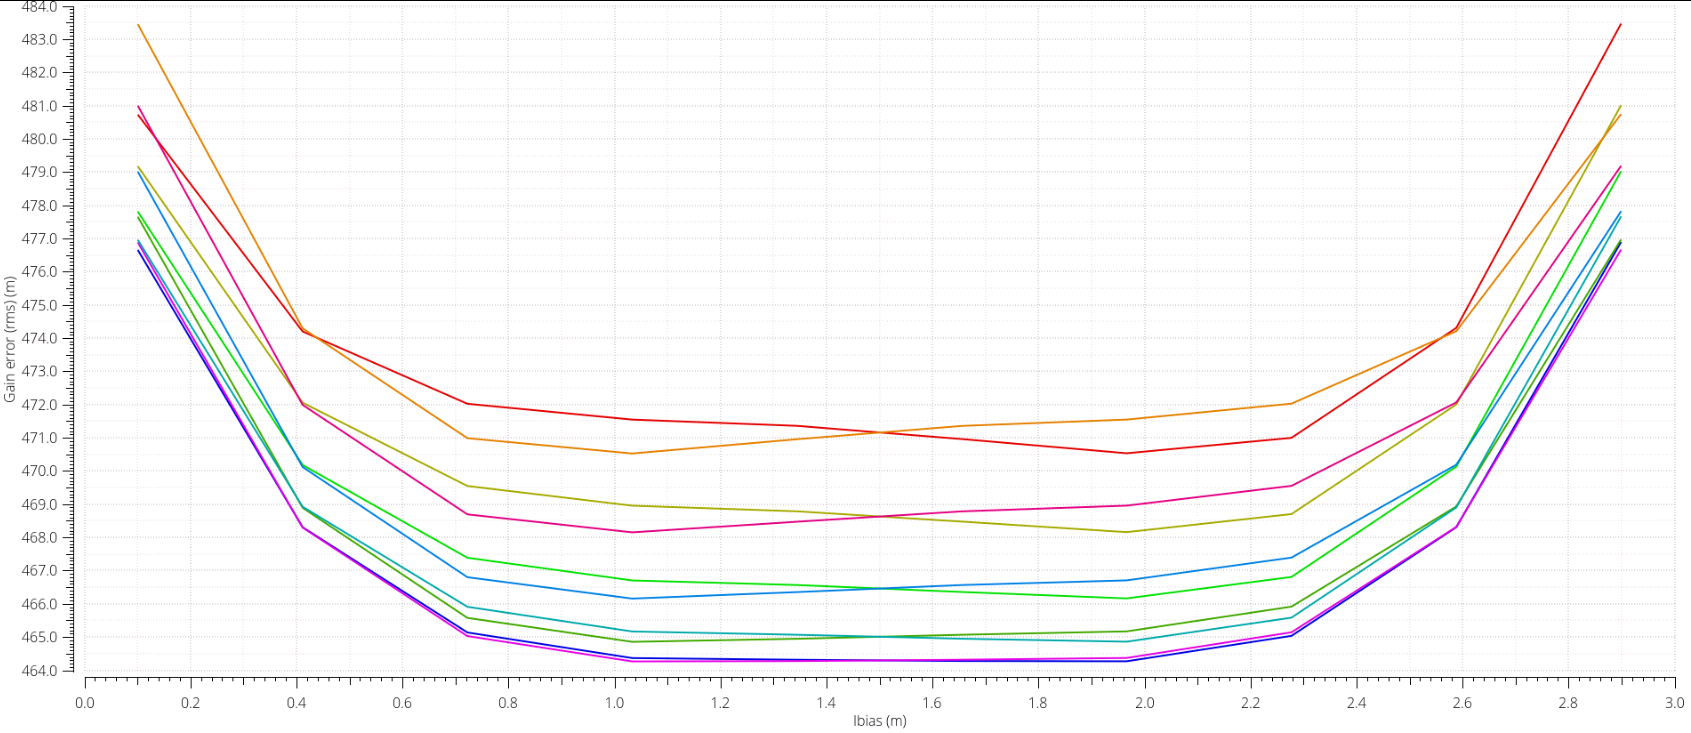
\includegraphics[width=\linewidth]{gain_error_rms.png}
  \caption{Odstupanje (rms) amplituda I/Q signala prema kontrolnoj struji}
  \label{fig:gain_error_rms}
\end{figure}

\begin{figure}[!htbp]
  \centering
  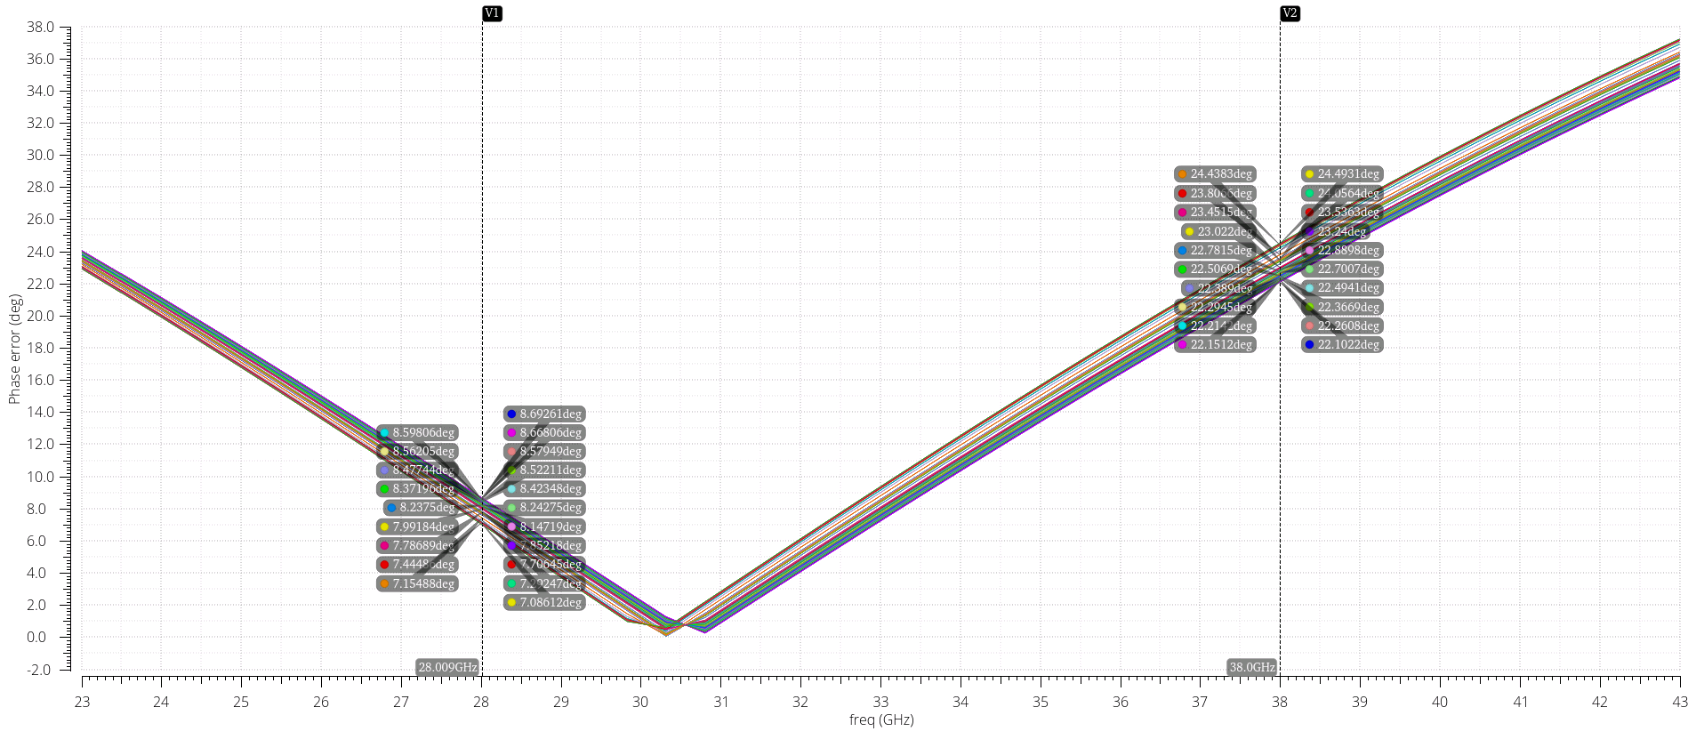
\includegraphics[width=\linewidth]{phase_error.png}
  \caption{Greška fazne razlike I/Q signala na opsegu učestanosti}
  \label{fig:phase_error}
\end{figure}

\begin{figure}[!htbp]
  \centering
  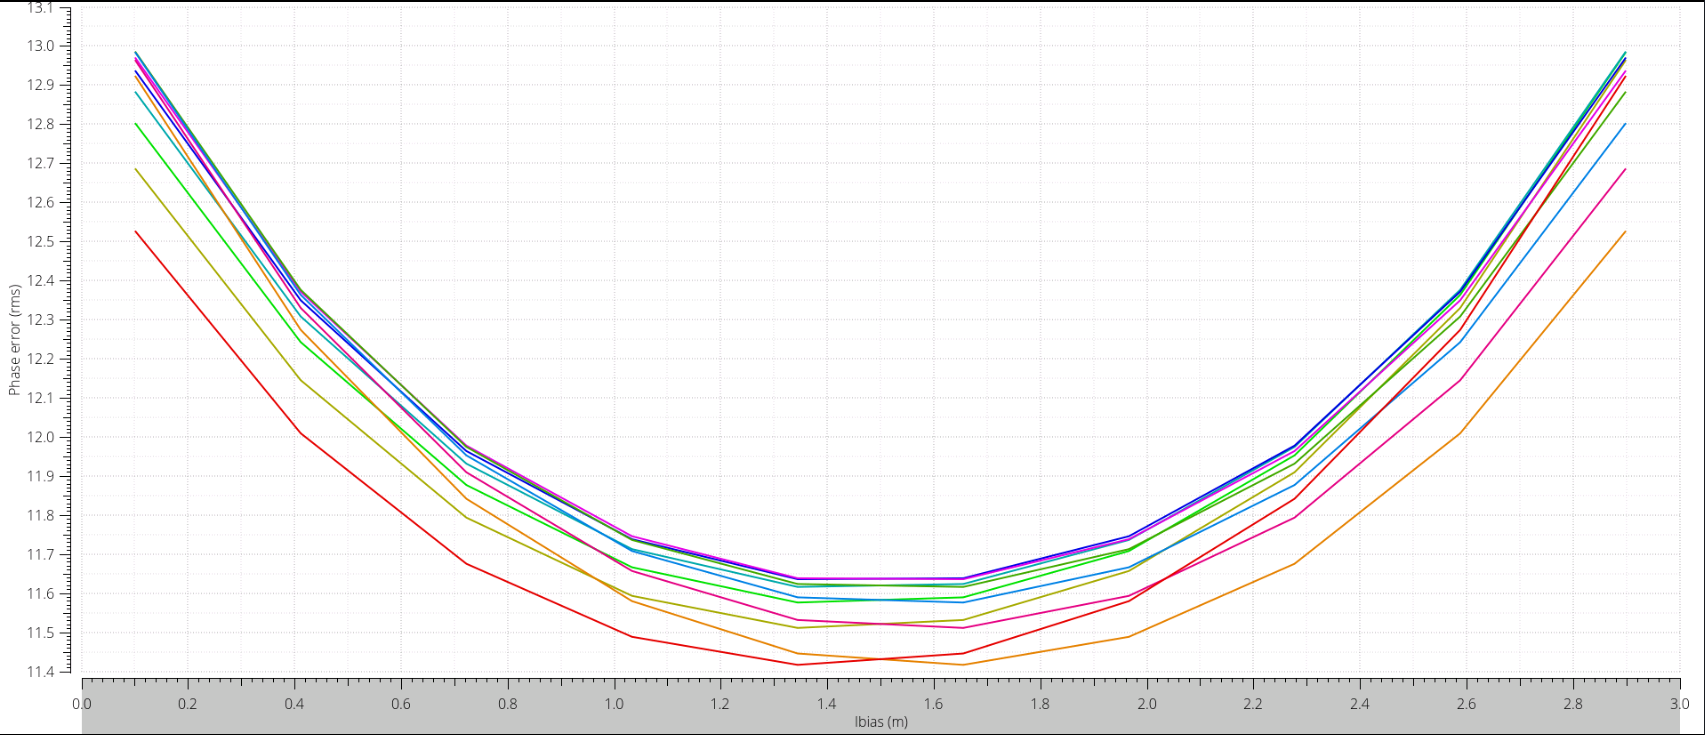
\includegraphics[width=\linewidth]{phase_error_rms.png}
  \caption{Odstupanje (rms) greške fazne razlike prema kontrolnoj struji}
  \label{fig:phase_error_rms}
\end{figure}

\begin{figure}[!htbp]
  \centering
  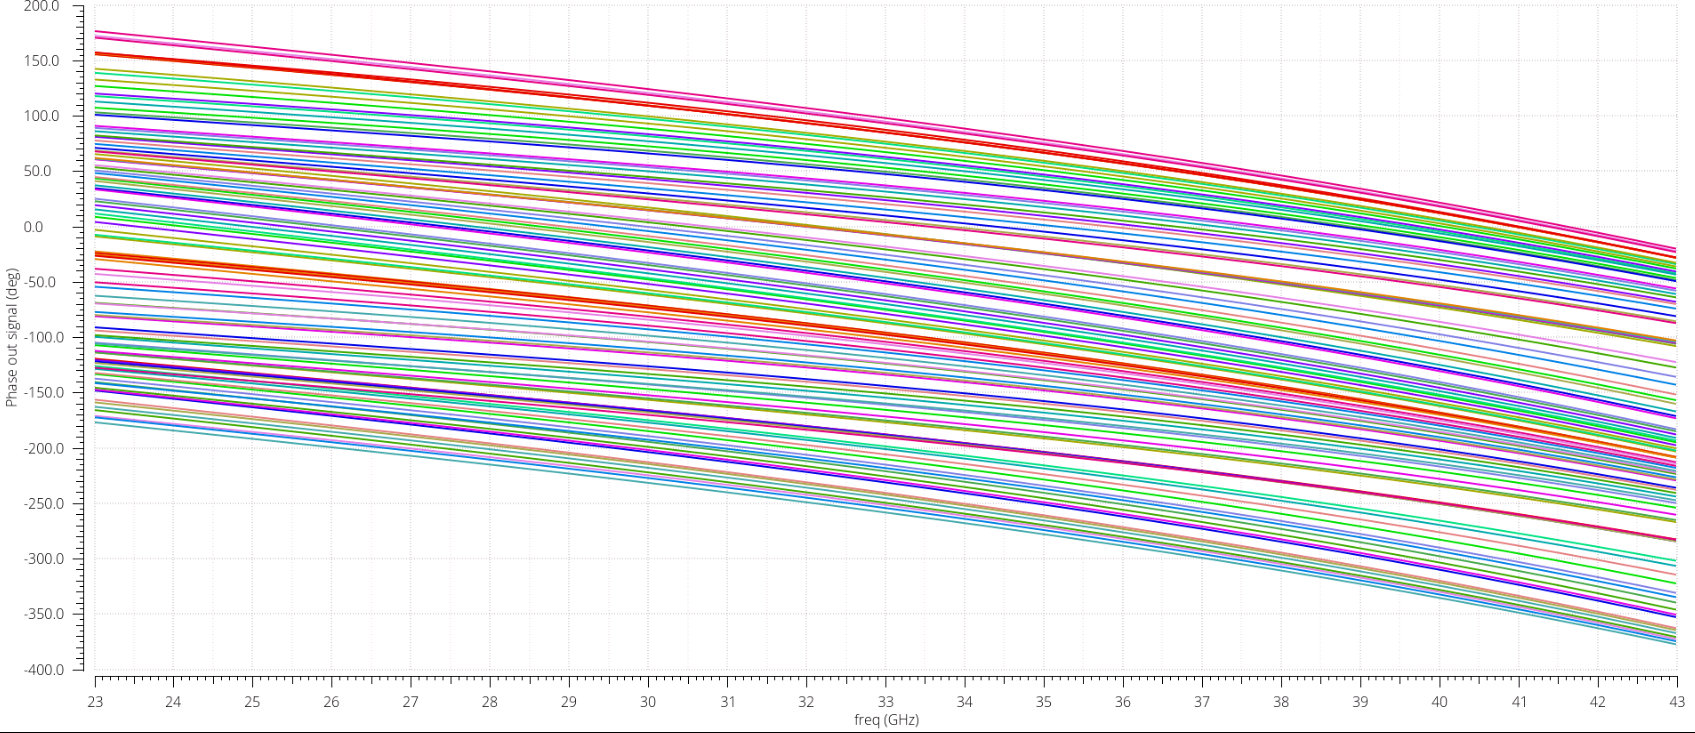
\includegraphics[width=\linewidth]{phase_out_signal.png}
  \caption{Opseg kontrole faze na izlazu vektor modulatora}
  \label{fig:phase_out_signal}
\end{figure}

\begin{figure}[!htbp]
  \centering
  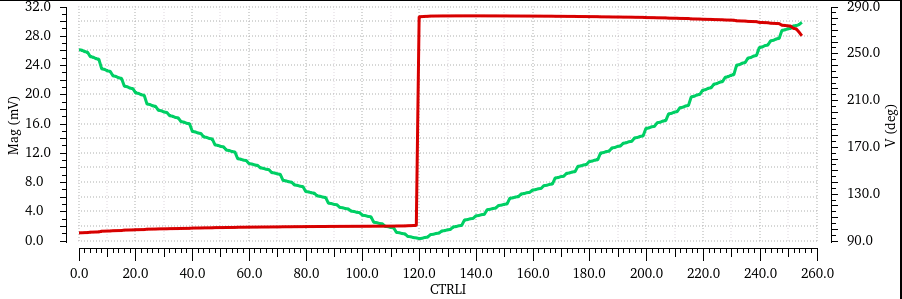
\includegraphics[width=\linewidth]{vga_linearity.png}
  \caption{Amplituda i faza izlaza jedne ćelije vektor modualtora}
  \label{fig:vga_linearity}
\end{figure}

\newpage

\section{Rezultati simulacija - druga iteracija}

S-parametri \textit{all-pass} filtra su ekstrahovani pomoću Momentum elektromagnetskog simulatora. Ostatak pomerača je simuliran sa \textit{schematic} blokovima za osnovne blokove DA kontrola, pojačavač promenljivog pojačanja, kolima za polarizaciju sa tehnološkim modelima, i sa idealnim elementima za kola za prilagođenje.


\begin{figure}[!htbp]
  \centering
  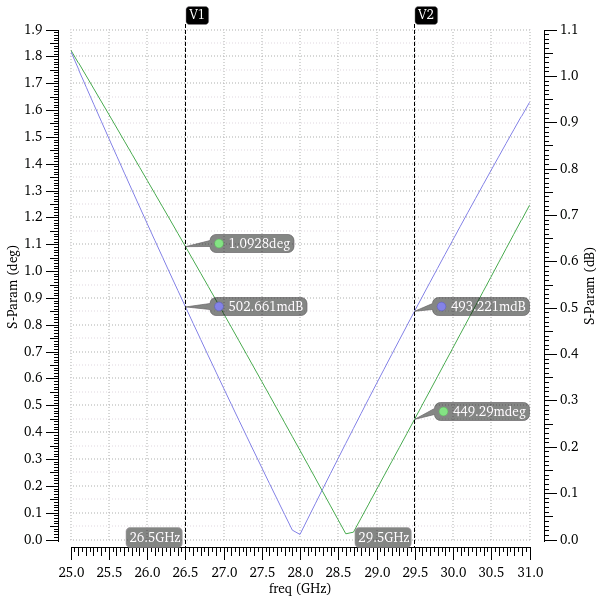
\includegraphics[width=\linewidth]{mag_phase_error_mom@28GHz.png}
  \caption{Amplitudska i fazna greška I i Q signala \textit{all-pass} filtra simuliranog \textit{Momentum}-u}
  \label{fig:mag_phase_error_mom@28GHz}
\end{figure}

% \begin{center}
%   \begin{tabular}{| c | c | c |} 
   
%     \hline
%     Parametar & Oznaka & vrednost\\ 
%     \hline
%     Debljina dielektrika & $h$ & $0.8 mm$  \\
%     \hline
%     Debljina metala  & $t$ & 35 $ \mu m $  \\
%     \hline
%     Relativna permitivnost & $\epsilon _r$ & 4.55  \\
%     \hline
%     Tangens gubitaka & $tan(\delta)$  & 0.02 \\
%     \hline
%     Specifična provodnost & $\sigma$ &  $58.8 MS/m $\\
%     \hline

%   \end{tabular}
% \end{center}


% \newpage

% An example of a floating figure using the graphicx package.
% Note that \label must occur AFTER (or within) \caption.
% For figures, \caption should occur after the \includegraphics.
% Note that IEEEtran v1.7 and later has special internal code that
% is designed to preserve the operation of \label within \caption
% even when the captionsoff option is in effect. However, because
% of issues like this, it may be the safest practice to put all your
% \label just after \caption rather than within \caption{}.
%
% Reminder: the "draftcls" or "draftclsnofoot", not "draft", class
% option should be used if it is desired that the figures are to be
% displayed while in draft mode.
%
%\begin{figure}[!t]
%\centering
%\includegraphics[width=2.5in]{myfigure}
% where an .eps filename suffix will be assumed under latex, 
% and a .pdf suffix will be assumed for pdflatex; or what has been declared
% via \DeclareGraphicsExtensions.
%\caption{Simulation results for the network.}
%\label{fig_sim}
%\end{figure}

% Note that the IEEE typically puts floats only at the top, even when this
% results in a large percentage of a column being occupied by floats.


% An example of a double column floating figure using two subfigures.
% (The subfig.sty package must be loaded for this to work.)
% The subfigure \label commands are set within each subfloat command,
% and the \label for the overall figure must come after \caption.
% \hfil is used as a separator to get equal spacing.
% Watch out that the combined width of all the subfigures on a 
% line do not exceed the text width or a line break will occur.
%
%\begin{figure*}[!t]
%\centering
%\subfloat[Case I]{\includegraphics[width=2.5in]{box}%
%\label{fig_first_case}}
%\hfil
%\subfloat[Case II]{\includegraphics[width=2.5in]{box}%
%\label{fig_second_case}}
%\caption{Simulation results for the network.}
%\label{fig_sim}
%\end{figure*}
%
% Note that often IEEE papers with subfigures do not employ subfigure
% captions (using the optional argument to \subfloat[]), but instead will
% reference/describe all of them (a), (b), etc., within the main caption.
% Be aware that for subfig.sty to generate the (a), (b), etc., subfigure
% labels, the optional argument to \subfloat must be present. If a
% subcaption is not desired, just leave its contents blank,
% e.g., \subfloat[].


% An example of a floating table. Note that, for IEEE style tables, the
% \caption command should come BEFORE the table and, given that table
% captions serve much like titles, are usually capitalized except for words
% such as a, an, and, as, at, but, by, for, in, nor, of, on, or, the, to
% and up, which are usually not capitalized unless they are the first or
% last word of the caption. Table text will default to \footnotesize as
% the IEEE normally uses this smaller font for tables.
% The \label must come after \caption as always.
%
%\begin{table}[!t]
%% increase table row spacing, adjust to taste
%\renewcommand{\arraystretch}{1.3}
% if using array.sty, it might be a good idea to tweak the value of
% \extrarowheight as needed to properly center the text within the cells
%\caption{An Example of a Table}
%\label{table_example}
%\centering
%% Some packages, such as MDW tools, offer better commands for making tables
%% than the plain LaTeX2e tabular which is used here.
%\begin{tabular}{|c||c|}
%\hline
%One & Two\\
%\hline
%Three & Four\\
%\hline
%\end{tabular}
%\end{table}


% Note that the IEEE does not put floats in the very first column
% - or typically anywhere on the first page for that matter. Also,
% in-text middle ("here") positioning is typically not used, but it
% is allowed and encouraged for Computer Society conferences (but
% not Computer Society journals). Most IEEE journals/conferences use
% top floats exclusively. 
% Note that, LaTeX2e, unlike IEEE journals/conferences, places
% footnotes above bottom floats. This can be corrected via the
% \fnbelowfloat command of the stfloats package.

\section{Zaključak}


TODO:

% \section*{Acknowledgment}
% The authors would like to thank...

% \renewcommand{\bibname}{Литература и радови}
\begin{thebibliography}{9}

\bibitem{ellinger10}
	Frank Ellinger, Uwe Mayer, Michael Wickert, Niko Joram, Jens Wagner, Ralf Eickhoff, Ignacio Santamaria, Christoph Scheytt, and Rolf Kraemer
	\textit{Integrated Adjustable Phase Shifters};
	IEEE Microwave magazine;
	October, 2010;
	DOI: 10.1109/MMM.2010.937730 \\

\bibitem{kim12}
 	Sang Young Kim, D.-W. Kang, K.-J. Koh, and G. M. Rebeiz,
	\textit{An Improved Wideband All-Pass I/Q Network for Millimeter-Wave Phase-Shifters};
	IEEE Transactions on Microwave Theory and Techniques, vol. 60, NO. 11, November 2012;
	April, 2012;
	DOI: 10.1109/TMTT.2012.2212027 \\
    
\bibitem{greenly05}
	Brandon Greenley, Raymond Veith, Dong-Young Chang, and Un-Ku Moon,
	\textit{A Low-Voltage 10-Bit CMOS DAC in 0.01-mm 2 Die Area};
	IEEE Transactions on Circuits and Systems—II: express briefs, vol. 52, NO. 5;
	May, 2005;
  DOI: 10.1109/TCSII.2005.843595 \\

\bibitem{wang17}
	Minghua Wang, Yu Liu, Zhiqiang Li, Xiaosong Wang, Muhamamad M Sarfraz, Yanbin Xiao, and Haiying Zhang, 
	\textit{A 6-bit 38GHz SiGe BiCMOS phase shifter for 5G phased array communications};
	IEICE Electronics Express, Vol.14, No.13, 1–10;
	May, 2017;
  DOI: 10.1587/elex.14.20170451 \\

\bibitem{zeki07}
	Ali Zeki, and Ali Toker,
	\textit{Tunable linear CMOS current mirror};
	Springer Science + Business Media, LLC 2007;
	January, 2007;
	DOI: 10.1007/s10470-007-9030-3 \\

\bibitem{chua98}
  M. Chua, and K. W. Martin,
  \textit{1GHz programmable analog phase shifter for adaptive antennas};
  in Proc. IEEE Custom Integr. Circuits Conf. pp. 71–74;
  May, 1998;
  DOI: 10.1109/CICC.1998.694909 \\






% \bibitem{homayoun13}
% 	A. Homayoun and B. Razavi,
%     \textit{Analysis of phase noise in phase/frequency detectors},
%     IEEE Trans. Circuits Syst. I ,
%     vol. 60, pp. 529-539,
%     Mar. 2013.
%     DOI: 10.1109/TCSI.2012.2215792 
    
% \bibitem{lee99}
% 	G. B. Lee, P. K. Chan and L. Siek,
%     \textit{A CMOS Phase frequency Detector for Charge Pump Phase-Locked Loop}, 
%     Nanyang Technological Univerisity, Singapore,
%     1999.
%     DOI: 10.1109/MWSCAS.1999.867710 

% \bibitem{chen10}
% 	W. H. Chen, M. E. Inerowicz and B. Jung,
%     \textit{Phase Frequency Detector With Minimal Blind Zone for Fast Frequency Acquisition}, 
%     IEEE Trans. Circuits Syst. II,
%     vol. 57, pp. 936-940, 
%     Dec. 2010.
%     DOI: 10.1109/TCSII.2010.2087951

% \bibitem{milosavljevi16}
% 	I. M. Milosavljević, Đ. P. Glavonjić, D. P. Krčum, L. V. Saranovac and V. M. Milovanović,
% 	\textit{A highly linear and fully-integrated FMCW synthesizer for 60 GHz radar applications with 7 GHz bandwidth}, 
% 	Springer, Analog Integrated Circuits and Signal Processing,
%     90(3), 591–604.
%     2016.
%     DOI: 10.1007/s10470-016-0910-2

% \bibitem{razavi96}
% 	B. Razavi,
% 	\textit{Monolithic Phase-Locked Loops and Clock Recovery Circuits: Theory and Design}, 
% 	Wiley-IEEE Press; 1st edition,
%     1996.
%     ISBN-13: 978-0780311497




\end{thebibliography}

% \begin{thebibliography}{1}

\twocolumn[
\begin{@twocolumnfalse}

\newpage

\end{@twocolumnfalse}]

\section{Pomerači faze reflektivnog tipa}

Centralni radovi: \\

[1] Mehdi Askari, Hooman Kaabi, Yousef S. Kavian \textit{"A 24 GHz reflective-type phase shifter with constant loss in 0.18 $\mu$m CMOS technology"}, AEU - International Journal of Electronics and Communications 69:1134-1142, May. 2015. DOI: 10.1016/j.aeue.2015.04.015 \\

[2] F. Ellinger, R. Vogt, and W. Bachtold, \textit{"Ultra compact reflective type phase shifter MMIC at C-band with 360$^o$ phase control range for smart antenna combining"}, IEEE J. Solid-State Circuits, vol. 37, no. 4, pp. 481–486, Apr. 2002. DOI: ??? \\


\section{Hibridni $3dB$-ski $90^o$-ni sprežnjak}


Hibridni sprežnjak je četvoroportni element sa jendim ulaznim portom, dva izlazna(gde su izlazi u fazi i sa pomerajem od $90^o$) i izolovani port. Hibridni sprežnjak se može napraviti pomoću vodova ili koncentrisanih elemenata (\textit{eng. lumped}). 



Radovi za razmatranje: \\

Pomerači faze reflektivnog tipa : \\

[29] F. Ellinger, R. Vogt, and W. Bachtold, “Compact reflective type phase
shifter MMIC for C-band using a lumped element coupler,” IEEE
Trans. Microwave Theory Tech., vol. 49, no. 5, pp. 913–917, May 2001. \\

[30] F. Ellinger, “A 15 GHz reflective type phase shifter MMIC fab-
ricated on 0.25 um SiGe BiCMOS technology,” in Proc. Int. Conf.
Telecommunication, May 2005, CD-ROM. \\

[31] H. Hayashi, M. Muraguchi, Y. Umeda, and T. Enoki, “A high-Q
broad-band active inductor and its application to a low-loss analog
phase shifter,” IEEE Trans. Microwave Theory Tech., vol. 44, no. 12,
pp. 2369–2374, Dec. 1996. \\


Šta su to aktivni kalemi? \\




% \bibitem{IEEEhowto:kim}



% \bibitem{IEEEhowto:pozar}
% D.~Pozar, \emph{Microwave Engineering}, \hskip 1em plus
%   0.5em minus 0.4em\relax Wiley, New Jersey, 2011.

% \bibitem{IEEEhowto:djordjevic}
% A.~Đorđević, D.~Tošić, \emph{Mikrotalasna tehnika}, \hskip 1em plus
%   0.5em minus 0.4em\relax Akademska misao, Beograd, 2006.

% \bibitem{IEEEhowto:ilic}
% M.~Ilić, S.~Savić, \emph{Mikrotalasna elektronika}, \hskip 1em plus
%   0.5em minus 0.4em\relax Akademska misao, Beograd, 2016.

% \end{thebibliography}

% biography section
% 
% If you have an EPS/PDF photo (graphicx package needed) extra braces are
% needed around the contents of the optional argument to biography to prevent
% the LaTeX parser from getting confused when it sees the complicated
% \includegraphics command within an optional argument. (You could create
% your own custom macro containing the \includegraphics command to make things
% simpler here.)
%\begin{IEEEbiography}[{\includegraphics[width=1in,height=1.25in,clip,keepaspectratio]{mshell}}]{Michael Shell}
% or if you just want to reserve a space for a photo:

% \begin{IEEEbiography}{Michael Shell}
% Biography text here.
% \end{IEEEbiography}

% \begin{IEEEbiography}{Zhengyu Peng}
% Biography text here.
% \end{IEEEbiography}

% % if you will not have a photo at all:
% \begin{IEEEbiographynophoto}{John Doe}
% Biography text here.
% \end{IEEEbiographynophoto}

% % insert where needed to balance the two columns on the last page with
% % biographies
% %\newpage

% \begin{IEEEbiographynophoto}{Jane Doe}
% Biography text here.
% \end{IEEEbiographynophoto}

% You can push biographies down or up by placing
% a \vfill before or after them. The appropriate
% use of \vfill depends on what kind of text is
% on the last page and whether or not the columns
% are being equalized.

%\vfill

% Can be used to pull up biographies so that the bottom of the last one
% is flush with the other column.
%\enlargethispage{-5in}

% that's all folks
\end{document}
